\documentclass[leqno]{article}
%%%%%%%%%%%%%%%%%%%%%%%%%%%%%%%%%%%%%%%%%%%%%%%%%%%%%%%%%%%%%%%%%%%%%%%%%%%%%%%%%%%%%%%%%%%%%%%%%%%%%%%%%%%%%%%%%%%%%%%%%%%%%%%%%%%%%%%%%%%%%%%%%%%%%%%%%%%%%%%%%%%%%%%%%%%%%%%%%%%%%%%%%%%%%%%%%%%%%%%%%%%%%%%%%%%%%%%%%%%%%%%%%%%%%%%%%%%%%%%%%%%%%%%%%%%%
\usepackage{indentfirst}
\usepackage{amsfonts}
\usepackage{amsmath}
\usepackage{amssymb}
\usepackage[doublespacing]{setspace}
\usepackage{sectsty}
%\usepackage{footmisc}
\usepackage{fullpage}
\usepackage[justification=centering,textfont={sc},labelfont={rm}]{caption}
%\usepackage{varioref}
\usepackage{graphicx}
%\usepackage{natbib}
%\usepackage{titling}
\usepackage[hidelinks]{hyperref}
\usepackage{booktabs}
\usepackage[flushleft]{threeparttable}
\usepackage{dcolumn}
\usepackage[input-symbols = ()]{siunitx}
\usepackage{pdflscape}
\usepackage{subcaption}
\usepackage{placeins}
\usepackage{titlesec}
\usepackage{ragged2e}
\usepackage[natbib, maxcitenames=3, maxbibnames=11, style=authortitle, citestyle=authoryear-comp, backend=bibtex, eprint=false, url=false]{biblatex}

% break up long URL at hyphens
\def\UrlBreaks{\do\/\do-}

% For reference
\renewbibmacro{in:}{}
\DeclareFieldFormat{pages}{#1}
\DeclareFieldFormat{note}{#1,}
\AtEveryBibitem{
	\clearfield{number}
	\clearfield{series}
	\clearfield{doi}
	\clearfield{type}}
\renewbibmacro*{publisher+location+date}{%
	\printtext[parens]{% ADDED
		\printlist{location}%
		\iflistundef{publisher}
		{\setunit*{\addcomma\space}}
		{\setunit*{\addcolon\space}}%
		\printlist{publisher}%
		\setunit*{\addcomma\space}%
		\usebibmacro{date}%
	}% ADDED
	\newunit}

\sectionfont{\normalfont\scshape\centering}
\renewcommand{\thesection}{\Roman{section}.}
\renewcommand{\thesubsection}{\thesection\Alph{subsection}.}
\subsectionfont{\itshape\mdseries}
\renewcommand{\thesubsubsection}{\arabic{subsubsection}.}

\titleformat{\subsubsection}[runin]% runin puts it in the same paragraph
	{\itshape}% formatting commands to apply to the whole heading
	{\thesubsubsection}% the label and number
	{0.5em}% space between label/number and subsection title
	{}% formatting commands applied just to subsection title
	[.]% punctuation or other commands following subsection title

\titlespacing{\subsubsection}{\parindent}{*2}{\wordsep}

\captionsetup[table]{
	labelsep=newline,
	justification=centering,
	singlelinecheck=false,
	textfont=normalfont
}

\captionsetup[figure]{
	labelsep=newline,
	justification=centering,
	singlelinecheck=false,
	textfont=normalfont
}


\sisetup{
	detect-all,
	round-integer-to-decimal = true,
	group-digits             = true,
	group-minimum-digits     = 3,
	round-mode				 = off, 
	round-precision			 = 3,
	group-separator          =  {,},
	table-align-text-pre     = false,
	table-align-text-post    = false,
	group-digits			 = integer,
	input-signs              = + -,
	input-symbols            = {*} {**} {***},
	input-open-uncertainty   = ,
	input-close-uncertainty  = ,
	retain-explicit-plus
}


%\makeatletter
%\def\@biblabel#1{\hspace*{-\labelsep}}
%\renewenvironment{thebibliography}[1]
% {\section*{\refname} \@mkboth{\MakeUppercase\refname}{\MakeUppercase\refname} \list{\@biblabel{\@arabic\c@enumiv}} {\singlespacing
% \settowidth\labelwidth{\@biblabel{#1}} \setlength{\itemsep}{0pt plus 1pt} \leftmargin\labelwidth
% \advance\leftmargin\labelsep
% \@openbib@code
% \usecounter{enumiv} \let\p@enumiv\@empty
% \renewcommand\theenumiv{\@arabic\c@enumiv}} \sloppy
% \clubpenalty4000
% \@clubpenalty \clubpenalty
% \widowpenalty4000 \sfcode`\.\@m}
% {\def\@noitemerr
% {\@latex@warning{Empty `thebibliography' environment}} \endlist}
%\makeatother

\makeatletter
%\renewcommand\@makefnmark{\mbox{\textsuperscript{\normalfont\@thefnmark}}}
%\renewcommand\@makefntext[1]{\indent\makebox[2.5em][r]{\@thefnmark.\,}#1}
\if@titlepage
  \renewenvironment{abstract}{      \titlepage
      \null\vfil
      \@beginparpenalty\@lowpenalty
      \begin{center}        \@endparpenalty\@M
      \end{center}}     {\par\vfil\null\endtitlepage}
\else
  \renewenvironment{abstract}{      \if@twocolumn
      \else
        \small
        \begin{center}        \end{center}      \fi}
      {\if@twocolumn\else\endquotation\fi}
\fi
\renewcommand\thetable{\@Roman\c@table}
\renewcommand\tablename{TABLE}
\renewcommand\thefigure{\@Roman\c@figure}
\renewcommand\figurename{\textsc{Figure}}
\makeatother

%\labelformat{equation}{(#1)}

%
%\makeatletter
%\DeclareRobustCommand\citepos
%{\begingroup
%	\let\NAT@nmfmt\NAT@posfmt% ...except with a different name format
%	\NAT@swafalse\let\NAT@ctype\z@\NAT@partrue
%	\@ifstar{\NAT@fulltrue\NAT@citetp}{\NAT@fullfalse\NAT@citetp}}
%\let\NAT@orig@nmfmt\NAT@nmfmt
%\def\NAT@posfmt#1{\NAT@orig@nmfmt{#1's}}
%\makeatother

\makeatletter
\@fpsep\textheight
\makeatother


\addbibresource{cdg.bib}

\begin{document}

\title{\uppercase{Making lemonade from lemons: Taxi drivers' response to cancellations and no-shows}\thanks{%
We gratefully acknowledge funding from Singapore Ministry of Education Social Science Research Thematic Grant, MOE2016-SSRTG-059, SPIRE. We are very grateful to one of the leading taxi companies in Singapore for providing us with the data for this research, and deeply indebted to its management team for sharing with us their insights on the taxi industry. The authors can be contacted at \href{mailto:bizdhl@nus.edu.sg}{\textit{bizdhl@nus.edu.sg}}, \href{mailto:bizcj@nus.edu.sg}{\textit{bizcj@nus.edu.sg}} and \href{mailto:bizyaod@nus.edu.sg}{\textit{bizyaod@nus.edu.sg}}}}

\author{%
\begin{tabular}{c}
\textsc{Hai Long Duong} \\ 
\textsc{Junhong Chu} \\ 
\textsc{Dai Yao}%
\end{tabular}
}

\date{}

\maketitle

\begin{abstract}
We study the impact of booking cancellations and passenger no-shows on taxi drivers' labor supply and productivity in Singapore's taxi industry. We employ a novel large dataset that covers three months of taxi bookings and street hail trips for one of the leading taxi operators in Singapore. Our analysis shows that drivers work longer and earn more per hour following cancellations or no-shows, as if they strive to make up for the loss from such adverse actions. Interestingly, working longer and increasing productivity are substitutable rather than complementary devices, and are chosen by taxi drivers in their own favor: More experienced drivers, with better job search skills than less experienced drivers, tend to work more diligently to increase productivity; solo drivers, with more flexible schedule than sharing drivers, tend to work more hours. Furthermore, these effects are strong in the immediate following hour and afterward fade away. Our results demonstrate the resiliency of platform markets and shed new light on how service providers react to negative shocks due to changes in customers' needs. \textit{JEL} Codes: J22, J24, D91.
\end{abstract}

%suggested JEL: J22 Time Allocation and Labor Supply; J24 Human Capital; Skills; Occupational Choice; Labor Productivity; D91 Role and Effects of Psychological, Emotional, Social, and Cognitive Factors on Decision Making

%TCIMACRO{%
%\TeXButton{Titlepage formatting}{\thispagestyle{empty}\setcounter{page}{0}}}%
%BeginExpansion
%\thispagestyle{empty}\setcounter{page}{0}%
%EndExpansion
\newpage 


\section{Introduction}
%After receiving rejections from journal editors, do academic researchers give up, or do they put in even more effort to better the chance of acceptance in the future? After machine breakdowns, do factory workers get more distressed, or do you become more motivated to continue the work? Does losing at halftime demoralize basketball teams, or does it make them more competitive in the second half? After a booking is cancelled, or a passenger fail to show up, do taxi drivers?

Negative shocks are an integral part of our lives: Researchers' articles are rejected by editors, factory workers are unable to work due to machine breakdowns, and taxi drivers' bookings get cancelled by riders. People have different reactions to and adopt different coping strategies for these shocks. On one hand, negative shocks typically generate negative emotions, which can further aggravate the situation; for example, \citet{cai2017recover} find that machine breakdowns not only render workers unable to work on the same day, but also decrease their productivity on the following day. On the other hand, if well managed, adverse outcomes can be significantly reduced and even reversed. For instance, \citet{berger2011can} find that in professional basketball, losing by one point at half-time actually increases the team's chance of winning the game.

In service sectors, a common negative shock is change in customers' needs: Customers may cancel their bookings or fail to show up, and the time and resources spent in preparation for their service would go to waste. Cancellations and no-shows (referred to as C\&NSs hereafter) are encountered not only by traditional service providers such as hotels, airlines, hospitals, etc., but also by workers in many emerging platforms and sharing economies such as ride-sharing, home-sharing, peer-to-peer renting, etc. C\&NSs are especially relevant for the service providers in these emerging sectors, due to the sheer volume of spot transactions generated by the large number of small independent agents these markets help to connect. More than ever, dealing with C\&NSs is part of the daily routine for workers in these sectors.

This paper studies how taxi drivers in Singapore cope with booking cancellations and passenger no-shows. C\&NSs, from the drivers' perspective, are adverse events they cannot control. In addition to the possible negative impact on the individual's mood, the immediate consequence is that drivers waste time and mileage driving to the pickup point and waiting for the passenger, which presumably affects their earnings negatively. Surprisingly, however, we find that the drivers in our data tend to be less likely to stop work and instead generate higher earnings in the hour following a C\&NS. These results are robust even after taking into account the effects of various factors, including market conditions and driver heterogeneity; it seems that drivers respond to the adverse event of a C\&NS by  working harder and more diligently, as if they are striving to compensate for the loss from such events. This coping strategy reduces, and sometimes even reverses, the negative impacts that C\&NSs have on overall earnings.

%Cross-side interactions are an important aspect of platform economies. 
%It is the need to interact with ever more agents from the other side that gives rise to the presence of cross-network externalities, which are a defining feature of platforms \citep{armstrong2006competition,rysman2009economics,sriram2015platforms,chu2016quantifying}. 
%In fact, \citet{hagiu2015multi} argue that it is the ability to enable direct interactions between multiple sides that differentiates multi-sided platforms from other forms of business such as resellers and vertically integrated firms. 

%Although there is a large literature on platform economics, pioneered by \citet{rochet2003platform}, existing works \citep{nair2004empirical,ohashi2003role, seamans2013responses,clements2005indirect,rysman2004competition,sun2016beyond,shriver2015network,pattabhiramaiah2017rising}\footnote{See \cite{rysman2009economics} and \citet{sriram2015platforms} for a review.} have focused mainly on the \emph{aggregate} effects of these interactions, and the main variable of interest is often the total number of agents on either side.
%These aggregate numbers can be viewed as a summary statistic of the volume of interactions occurring in the market, albeit a very crude one.
%In fact, not all actions in the market are of the same nature, nor should we expect their effects to have similar magnitudes or even direction. For example, in television advertisement, \citet{wilbur2008two} finds that, while advertisers value TV advertising hours, viewers tend to be averse to them; and in consumer-to-consumer platforms, \citet{chu2016quantifying} show that the installed base of sellers has a much larger effect on the growth of buyers than vice versa.
%%Existing literature has focused mainly on the aggregate effects of these interactions, identifying the impacts of the size of one side of the platform on the other side, as well as on the market as a whole\footnote{CD players (Gandal et al., 2000), automatic clearing house (Ackerberg and Gowrisankaran, 2006), advertising (Rysman, 2004; Wilbur, 2008), C2C (Chu and Manchanda, 2013).}.
%This asymmetry in the aggregate effects underscores the complexity of the behavioral impacts of each individual interaction, and thus it calls for more detailed studies into the nature of these interactions from a micro perspective.
%
%%However, to the best of our knowledge, very few studies have looked at the microeconomics of cross-side interactions.
%A few studies have also examined the microeconomics of cross-side interactions. \citet{lin2015home} study the home bias between borrowers and lenders in an online crowd-funding market,  
%\citet{ma2015squeaky} study the interactions between customers and firms over social media, \citet{zhang2017meet} study buyer and seller bargaining in an online consumer-to-consumer platform, \citet{chintagunta2017quantifying} investigate the value of seller location in an online consumer-to-consumer platform, and \citet{dai2018multistep} examine the multi-stage transaction process in a peer-to-peer car rental platform.
%%Even in a small number of cases where individual interactions are examined, such as , and  
%The focus of these studies has been on mutually beneficial interactions in successful transactions between the two sides. 
%Though some studies \citep{edelman2017racial} demonstrate racial discrimination on platforms, they are often based on the list prices, not actual transactions. 
%%Even in a small number of cases where individual interactions are examined, such as \citet{zhang2017meet} who study buyer and seller bargaining in an online consumer-to-consumer platform, and \citet{lin2015home} who study the home bias between borrowers and lenders in an online crowdfunding market, the focus has been on mutually beneficial interactions in successful transactions between the two sides. 
%%Understanding how individual action from one side of the market affects individuals on the other side not only provides behavioral theories with new tests and insights from the new emerging context of platform economics, but also helps researchers develop micro foundation when analysing the drivers of cross-network effect.
%In this paper, we ask how an individual's adverse action, particularly failed transaction, from one side affects the behaviors of individuals on the other side in a two-sided market.

%The market that we examine is Singapore's taxi industry and the interactions that we focus on are booking cancellations and passenger no-shows. 
The taxi industry has been a subject of great interest to economists due to its special work arrangement, which enables empirical tests of various competing economic theories. The typical arrangement in Singapore is for the taxi operator to lease cabs to drivers using specific rate schemes, and drivers freely choose how long to work each day. Put another way, the taxi operator has ``sold the firm" to drivers, and each driver plays the role of a self-employed entrepreneur, internalizing into his own venture all of the costs and benefits of supplying labor. One feature of Singapore's taxi industry that differentiates it from the extensively studied New York City (NYC) yellow cab market is that it is very common for customers to book taxi services via telephone, SMS, the internet, and mobile apps, whereas in NYC cabs are mostly hailed on the street\footnote{A number of for-hire vehicle companies in NYC provide prearranged transport service, but the number of trips completed by these companies is relatively small compared to yellow cab trips (Taxi and Limousine Commission Factbook, 2016). Recently, several mobile apps such as Curb have been developed to allow yellow and green cabs in the city to accept bookings (see \url{https://www.theverge.com/2016/3/23/11294758/curb-app-taxi-hail-uber-nyc-verifone}).}. With the arrival of ride-sharing services such as Uber and Grab, customers in Singapore are becoming more accustomed to booking their rides, and taxi operators are increasingly promoting their own booking systems in order to remain competitive. In essence, Singapore's taxi industry is a combination of traditional taxi services and a modern ride hailing platform business.
%For this reason, Singapore's taxi industry lends itself nicely to the scope of multi-sided market research, since taxi operators here also play the role of a platform, connecting drivers and riders through their booking systems. 


There are two main reasons for our focus on booking cancellations and passenger no-shows as the negative shock of interest in this market.
First, conditional on market conditions and drivers' bidding for the bookings, C\&NSs are exogenous events from the drivers' perspective, as  
%because
these actions are entirely 
%dependent on 
customers' decisions. Moreover, the booking system provides nothing but 
%no demographic information about a driver to the customer except for 
the estimated time of arrival and the vehicle's plate number to the customer, and hence it is unlikely that customers' actions are influenced by driver characteristics such as gender, race, or age, as is common in other markets \citep{mejia2018transparency,cui2016discrimination,edelman2017racial,NBERw22776}. This enables clean identification of the effects of C\&NSs on driver behavior. In our analyses, we use a rich set of control variables and fixed effects to absorb the impacts of aggregate demand and supply conditions, as well as drivers' propensity to bid for a booking, and hence the estimated effects of C\&NSs reflect drivers' responses to customers' adverse actions.

Second,  C\&NSs are a relatively common phenomenon in many, if not all, services. While a large literature is devoted to them,  most studies \citep{moore2001time,liu2010dynamic,feldman2014appointment,zacharias2014appointment} have focused only on operational aspects and have largely ignored the behavioral effects of these actions, such as how they would impact workers' morale and motivation.
From an operational perspective, it is straightforward to see that C\&NSs generate lost sales, and the uncertainty associated with them entails the use of additional resources such as buffer time, stand-by personnel, rescheduling capacity, etc. which can be costly to service providers.
In this paper, we show that C\&NSs can also induce behavioral changes from agents on the supply side, and these changes may not always go in the same direction as the operational effects.
The  drivers in our study tend to make up for the negative operational effects caused by C\&NSs, and sometimes even reverse the sign of the effects.
These responses are likely even more profound on platforms that connect multiple small agents with each other.
Organizations that serve a large number of customers, such as airlines and hotel chains, may employ overbooking or other risk management tools to minimize the effects of such adverse actions.
In contrast, taxi drivers and other small independent service providers typically serve one customer at a time, and hence must absorb all of the risks and costs associated with the customer's actions.

%The third reason is that C\&NSs may generate externalities and have implications for cross-network effects. In most cases, as it is the case for the subjects of our study, customers are not penalized for their C\&NSs. They, however, generate real cost to the service providers -- taxi drivers in our case. Thus, the customers who cancel bookings or do not show up do not pay the full cost  of their actions, and hence they will tend to overdo it. Moreover, due to reallocation of the vehicles when the drivers try to reach the cancelled demand, these actions may distort the spatial distribution of taxicab supply over time, increasing search friction, which in turn can lead to longer waiting time for other customers in the market. In other words, the adverse actions from one side of the platform done to the agents on the other side may even generate indirect negative externalities on other agents from the same side. This can even create an additional layer of network effect on the platforms, since the more cancellations the customers make, the more mis-allocations the drivers have, the larger the search friction, the longer the expected waiting time, which leads to even more C\&NSs. Interestingly, our results suggest that the drivers actually respond in a way that offsets the negative impacts of C\&NSs, and hence keep these effects from spilling over the network. Within the scope of this paper, we do not analyse this aspect of C\&NSs, but hope that this brief discussion can motivate further research on the topic.

With the rise of the sharing economy, interactions between independent individuals in the marketplace are becoming ever more ubiquitous. Services in the sharing economy often take advantage of information and communication technologies to enable matching among a large number of individual agents, and rely on spot transactions rather than long-term contracts to facilitate flexible arrangements between agents. As a result,  participants in these markets are more exposed to the consequences of the counterparty's actions than those under protection from incumbent organizations and long-term contracts. Essentially, the sharing economy enables individuals to become ``taxi drivers" in the respective industry. This allows them to set their own schedules, but they must also accept all of the idiosyncrasies related to income and working environment when interacting with customers, in the same manner as traditional taxi drivers. Coping with negative shocks throughout the work day is becoming an important aspect of employment in the new economy.

This paper focuses on two service provider behaviors: labor supply and productivity. First, we ask how C\&NSs affect drivers' propensity to end their shifts and how long they continue to work following a C\&NS.  Second, we ask how the rate of earnings and percentage of paid time---i.e., with a passenger on board---change after experiencing a C\&NS. Third, we investigate the dynamics of these effects, i.e., how drivers' responses change over time. Specifically, we examine how C\&NSs in the current hour affect driver behavior, not only in the current hour but also in  each of the subsequent hours. Fourth, we examine the interrelationship between the two behavioral adjustments, labor supply versus productivity, by examining heterogeneous effects among groups of drivers who have a comparative advantage in one type of adjustment. Specifically, we look at how solo drivers, who do not share their taxi with another driver and therefore have an advantage in terms of prolonging their working hours, adjust their labor supply; and how more experienced drivers, who have an advantage in terms of skill---and hence tend to be better at managing their productivity---adjust their  productivity. Analysis of these dynamics and heterogeneous effects will yield suggestive evidence about the underlying mechanisms that drive these behavioral responses.

We exploit a novel dataset provided by one of the leading taxi operators in Singapore, which covers three months of street hail trips and taxi bookings by more than 30,000 drivers, and comprises 34 million observations for the period December 1, 2016-February 28, 2017. To the best of our knowledge, this is the first taxi dataset of this size in a research study that contains detailed information about not only street hail trips and taxi bookings, but also C\&NSs.
%\footnote{\citet{agarwal2015singaporean} use a dataset with detailed real-time taxi location and status in Singapore over a period of one month. Presumably, with such information, a researcher could identify all bookings and back out their status. However, the authors do not make use of this information, since the paper's focus is on income targeting behavior.}. 

Our analysis shows that drivers work longer and earn more per hour following C\&NSs, apparently seeking to compensate for the loss from such adverse actions. Longer work hours and increased productivity can reverse the negative impact of cancellations, leading to a higher income for the shift. However, they can only fully offset the negative impact of no-shows on the shift income, due to more time wasted by no-shows. Interestingly, working longer and increasing productivity are substitutable rather than complementary devices, and are chosen by taxi drivers in their own favor: As noted above, more experienced drivers, with better job search skills than less experienced ones, tend to work more diligently to increase their productivity; and solo drivers, with a more flexible schedule than sharing drivers, tend to work more hours. Furthermore, these effects are strong in the first hour after a C\&NS and fade away afterward. 

Our paper makes the following contributions to the literature. First, it is the first to study workers' behavioral responses to C\&NSs in the service sector. This is related to the literature on the impacts of C\&NSs \citep{moore2001time,patrick2008reducing,norris2014empirical,feldman2014appointment}, but our focus is on the behavioral effects rather than the operational aspects of C\&NSs. The paper is also related to the literature on service quality management \citep{cohen2018frustration}, but our interest is in how workers cope with C\&NSs rather than customer satisfaction and retention. Second, the paper contributes to the literature on the labor supply of taxi drivers by providing additional empirical evidence for both neoclassical and income targeting behaviors in the new context of Singapore's taxi industry, and identifying new determinants of labor supply: booking cancellations and customer no-shows. Third, the paper contributes to the literature on two-sided markets, being among the first to study the (negative) interactions between agents on both sides of the market at a micro level.


The rest of the paper is organized as follows. Section II reviews related literature. The background of Singapore's taxi industry and an overview of the data are presented in Section III.  We report the main results in Section IV, 
%. We then present robustness checks and further discussion in Section V, 
and conclude with  managerial implications in Section V.

\section{Literature Review}

Our research is related to several strands of literature. First, the paper contributes to the growing literature on productivity and performance under stress and negative shocks. We focus on a common source of negative shocks in the service sector, C\&NSs, and how they affect service providers---in our case, taxi drivers. Second, the taxi industry and taxi drivers  have been studied extensively in the labor supply literature, and our paper draws several connections to this literature. Third, our research complements various studies in operations research and management that have examined the operational impacts of C\&NSs, especially on hospital and clinic appointments. Lastly, among studies on two-sided markets, our paper is one of the first to investigate the implications of adverse interactions between agents from both sides of the market at a micro level.


\subsection{Coping under stress and/or negative shocks}

Negative shocks can generate pressure, frustration, change in motivation, or other emotional responses and affect performance.  These responses can be negative, which exacerbates the situation even further, especially if the original impact of the shock is large. For instance, in the context of factory production, \citet{cai2017recover} find that machine breakdowns decrease worker productivity on the following day, which is likely to be caused by negative emotions and increased cautiousness. However, if the shock is modest, it can sometimes be managed and coped with, such that the negative effects can even be reversed. In sports, \citet{berger2011can} analyze 18,000 professional basketball games and find that being slightly behind at half-time actually increases the winning percentage. The authors attribute this phenomenon to the goal-setting behaviors and motivational factors that seem to be consistent with prospect theory. In a laboratory experiment study, \citet{buser2016impact}  finds that losing a competition tends to increase willingness to seek further challenges, and this effect is more prevalent in men than women; it is worth noting that Singapore's taxi drivers are predominantly male, with only 2\% female drivers. \citet{cai2016gender} study the gender gap in \emph{gaokao} (China's competitive and high stake national college entrance examination) and find that male students outperform females on the actual examination relative to their performance on the mock examination. Interestingly, they also find that male students outperform themselves on the actual examination, relative to the mock examination, if their mock-examination score is slightly lower than the cutoff point. 


The focus of our study is on a commonly encountered negative shock, C\&NSs, in a market with a large number of small independent service providers.
Our findings are consistent with the results in this literature: C\&NSs are small negative shocks that taxi drivers encounter throughout the day, and can actually improve drivers' willingness to take on more job opportunities and increase their productivity.

\subsection{Cancellations and no-shows}

C\&NSs have been studied in other contexts, most notably in hospital and clinic appointments. A strand of the literature has studied the determinants of C\&NS decisions by customers, including weather, age, transportation difficulties, new versus returning patients, and modes of scheduling, among others \citep{norris2014empirical}. \citet{moore2001time} quantify the revenue shortfall due to no-shows at a family practice clinic as 3\%-14\%. Operations research literature has examined how to optimize booking and scheduling systems to reduce the effect of C\&NSs \citep{feldman2014appointment,patrick2008reducing}.

Our paper contributes to this literature by providing evidence that the effects of C\&NSs can go beyond their impact on the operational flow of the system; they may even change how human actors in the system behave. This also suggests that without taking into account the behavioral responses from human actors, any estimates of the operational effects of C\&NSs are likely to be biased. For example, if taxi drivers try to offset the negative impacts of booking C\&NSs, the taxi operator may not be able to observe any changes in system-wide earnings or utilization, and could underestimate the true operational impacts of those actions. Our results highlight the need to take into account the behavioral effects of cross-side interactions when designing and evaluating platform performance.


\subsection{Labor supply}
The labor supply of taxi drivers has been studied extensively in labor economics. The time flexibility that taxi drivers enjoy, coupled with the high fluctuations in daily wages they experience, makes them ideal subjects for testing the implications of competing labor supply models. In their seminal paper, \citet{camerer1997labor} find that the wage elasticity of work hours among NYC drivers is negative, which is at odds with neoclassical theory but consistent with income targeting behavior. \citet{crawford2011new} formalize this idea with a structural model, building on \citeauthor{kHoszegi2006model}'s \citeyear{kHoszegi2006model} concept of reference dependent preference, and find the presence of both income targeting and hour targeting behaviors among NYC drivers. \citet{farber2005tomorrow} criticizes \citeauthor{camerer1997labor}'s econometrics and proposes a discrete choice stopping-time model for labor supply. He finds that hours of work affect decisions to stop work, but---consistent with neoclassical theory---income does not. \citet{farber2015you} exploits a large dataset with over 100 million taxi trips in NYC and finds that even though income slightly affects labor supply decisions, hours of work are still the more important factor, and neoclassical effects seem to dominate income targeting effects. \citet{martin2017quit} uses similar data and finds evidence of not only loss aversion, but also diminishing sensitivity to loss among taxi drivers in NYC and San Francisco, which is consistent with prospect theory \citep{kahneman1979prospect}. 

The literature has evolved substantially over time  in terms of both methodology and data quality. The methodology has gradually moved away from ordinary least squares and instrumental variables regressions of working hours on wage  at shift level \citep{camerer1997labor}, which are prone to measurement errors, toward discrete choice models of labor supply decisions at trip level \citep{farber2005tomorrow,farber2015you,crawford2011new,martin2017quit}. Researchers also increasingly leverage more complete and higher-quality data, thanks to the availability of large administrative datasets such as the NYC Taxi and Limousine Commission (TLC) dataset. A number of recent studies have also looked at app-based ride-sharing services such as Uber, Grab, and Lyft, using the large volume of data generated by these platforms and their ability to price trips dynamically. \citet{chen2015dynamic} find that U.S. Uber drivers work more during a price surge, which is consistent with neoclassical theory; \citet{chen2017value} study the benefits of work flexibility among Uber drivers; and \citet{hall2017labor} combine Uber data and TLC yellow cab taxi data to study short- and long-run effects of fare changes on drivers' wages and labor supply. However, since the focus of this literature has been on testing whether taxi drivers' labor supply decisions are consistent with neoclassical economic theory or income targeting theory, it has not investigated how taxi drivers respond to the adverse actions of customers, which is the focus of our paper.

Our paper draws on this literature in two ways. First, the data we use are similar to the data used in the most recent work in this literature, with one notable difference: Our data also include bookings, cancellations, and no-shows, which enable us to employ similar methodology in the literature for data analysis and shed new light as well. Second, we also focus on labor supply, and in line with findings from this literature, we carefully control for neoclassical labor effects and income targeting effects when necessary. We also contribute to this literature in two ways. First, we provide more evidence for both neoclassical labor supply effects and income targeting effects among taxi drivers in the new context of Singapore's taxi industry. Second, we identify  additional determinants of taxi drivers' labor supply: booking cancellations and passenger no-shows.

\subsection{Two-sided markets}

\citet{armstrong2006competition,caillaud2001competing, caillaud2003chicken,rochet2003platform, rochet2006two} provide theoretical frameworks for two-sided markets. A common feature of these studies is the presence of cross-network effects, by which the benefit of participating in the platform depends on the number of agents on the other side of the platform. More recent empirical literature has focused on identifying the presence and magnitude of cross-network effects, investigating platform behavior---such as pricing structure, openness, competition, and innovation, among others---and examining policy implications \citep{rysman2009economics, sriram2015platforms}.

Our paper contributes to this literature in the following ways.  First, this is one of the few papers that examine the behavior of market participants, in contrast to the usual focus on the intermediary's behaviors. 
Second, our paper is also one of the first to study the effects of individual interactions---particularly adverse interactions---in two-sided markets at a micro level. Previous literature has largely focused on aggregate cross-network effects by investigating how the size of one side of the market influences the behavior of agents on the other side. Our paper takes a micro-oriented approach to examine the individual interactions that comprise the network effects. Different from the literature that often  examines successful transactions \citep{zhang2017meet,lin2015home,chintagunta2017quantifying,dai2018multistep} or the literature on the impacts of platform failures (e.g., mobile app failures; \citep{narang2018impact}), we instead study failed transactions between the two sides. Surprisingly, we find that failed transactions are not always bad news for all parties involved; they can sometimes induce behavioral changes that improve efficiency and benefit the market.


\section{Industry Background and Data Description}


\subsection{Industry background}

Singapore is a city-state with 721 sq km in land area and 5.6 million residents as of 2017. As a popular tourist destination, the city receives more than 15 million visitors each year\footnote{\url{https://www.stb.gov.sg/statistics-and-market-insights/Pages/statistics-Visitor-Arrivals.aspx}}.
Singapore has one of the world's most extensive transportation networks, with 200 km of rail network\footnote{\url{https://data.gov.sg/dataset/rail-length}},
357 bus routes in operation\footnote{\url{https://data.gov.sg/dataset/public-transport-capacity-average-daily-km-travelled-and-bus-routes-in-operation?resource_id=77fb71a7-4e7b-4a2b-9b99-83a5770b3e8b}},
and total bus and rail ridership of 7.2 million per day\footnote{\url{https://www.gov.sg/news/content/the-straits-times---bus-rail-ridership-soars-to-new-high}}.
The total number of taxicabs at the end of February 2017 is 26,986, amounting to around 4,820 cabs per million residents. In contrast, New York City, with 783 sq km in land area and a population of 8.6 million, has 13,237 yellow taxicabs in operation\footnote{NYC added street hail livery service (Boros Taxi) in 2013, with 7,676 vehicles in operation at the end of 2015, but these taxis can only pick up passengers in the outer boroughs.}, for an average of about 1,540 cabs per million residents.

The taxi market in Singapore was liberalized in 2003, and new operators are allowed to enter the market. Currently, there are seven taxi operators 
%\footnote{\url{https://www.lta.gov.sg/content/ltaweb/en/public-transport/taxis\%20and\%20private\%20hire\%20cars/taxi-operators.html}} 
and two main ride-sharing services (Grab and Uber)\footnote{Grab acquired Uber's Southeast Asia business in March 2018, and the acquisition is pending approval by the Competition Commission of Singapore. During the period in our sample, the two companies operated independently.}. Only Singapore citizens with a Taxi Driver's Vocational License are allowed to work as taxi drivers in Singapore. Drivers can join as either hirer drivers or relief drivers. Hirer drivers lease cabs directly from the operators, and relief drivers arrange the lease privately with hirers.

All cabs in Singapore are fitted with electronic meters. Taxi fare structures are regulated but highly variable,
with various surcharges based on time and location of the trip. For standard taxis, the base fare consists of (1) a flag-down fare of 3.2 to 3.9 Singapore dollars (SGD, 1 SGD = 0.7 USD during the data period), 
%\footnote{One SGD was exchanged at around 0.7 USD during the sample period.}
(2) a variable distance rate of 22 to 25 cents for every 400 m in the first 10 km and 22 to 25 cents for every 350 m after 10 km of travel, and (3) a waiting time fare of 22 to 25 cents for every 45 seconds. Time-based surcharges can be as high as 50\% of the meter fare between midnight and 6:00 a.m. Location surcharges range from 2 to 5 SGD. Bookings incur a fixed fee, which varies with pick-up time, taxi type, and how far in advance the booking is made. For normal taxis, the booking fee is 3.3 SGD during peak hours (6:00 p.m. to midnight every day and 6:00 a.m. to 9:30 a.m. on weekdays) and 2.3 SGD during non-peak hours; however, it can be as high as 20 SGD for advance booking with Chrysler cabs. Bookings can be made through a number of channels, including mobile app, SMS, hotline, and web portal. In our sample, mobile apps are by far the most popular way to book a cab, accounting for more than 57\% of bookings.

The booking fee is a nontrivial portion of the total fare. The typical booking fee (3.3 SGD) equals 19\% of the total fare for an average booking trip (17.53 SGD, inclusive of the booking fee) or 23\% of the trip fare exclusive of the booking fee. Furthermore, there is no penalty for C\&NSs, which makes street hail trips much more cost effective for passengers, except for the uncertainty of these pickups. As a result, if a passenger, while waiting for the booking, sees an empty taxi passing by, it is likely that she will jump on the taxi and forgo the booking. By doing so, not only does she avoid paying the nontrivial booking fee, but also shorten the waiting time. Calling back to cancel the booking is optional, and hence this can result in either a cancellation or a no-show. Therefore, many C\&NS incidents are due to random encounters between the waiting passenger and an empty taxi on the street.

The taxi operator employs a booking bidding system. The booking process proceeds as follows. First, a passenger makes a booking via one of the available channels and provides relevant information such as pick-up location, drop-off location, and requested pick-up time. Second, the taxi operator broadcasts the booking to a number of nearby drivers. Third, drivers bid for the booking by stating how quickly they can reach the passenger. The driver with the best bid wins the booking and drives to the pickup location. During this process, the passenger can cancel the booking at any time and the driver is informed of the cancellation instantly. Otherwise, the driver proceeds to the indicated pickup point and, if the passenger shows up, drives him/her to the destination. There is no compensation to drivers for C\&NSs.

\subsection{Data description and model-free evidence}

\subsubsection{Data description}
Each observation in the data corresponds to either a street hail trip or a booking. For street hail trips, we observe the start time and end time, pickup and destination postal code, 
%\footnote{In Singapore, each building has a unique 6-digit postal code and designated pick-up areas.}
 travel distance, total fare, vehicle ID, and driver ID. For bookings, we observe the booking time, requested pickup time, booking channel, booking status,  ID of the assigned vehicle, and, if the booking is completed, all information on the trip mentioned above. Bookings, with completed, failed, cancelled, or no-show status\footnote{``completed" indicates completed bookings, ``failed" indicates bookings for which the system failed to find a cab to assign to them, ``cancelled" indicates bookings that are cancelled by the passenger, either before or after the system assigns a cab to them, and ``no-show" indicates bookings in which the passenger did not show up.}, take up 27\% of  total observations: 76\% of all bookings are completed, 13\% are cancelled, 10\% are failed, and slightly more than 1\% are no-shows.

The data include 24,828,442 street hail trips and 9,114,421 bookings made between December 1, 2016 and February 28, 2017. During that period, 33,849 drivers were working and 17,468 vehicles were in operation\footnote{A 
%vehicle can be shared among multiple drivers, and a 
driver can drive multiple vehicles, although the great majority of drivers stick with one vehicle.}. Of the drivers, 98\% are males, 78\% are over the age of 50, and 84\% have worked for the company for more than two years. Around 11\% of all drivers are solo drivers, 35\% share a cab with one other driver, 30\% with two other drivers, and 24\% with at least three other drivers.

Following the literature \citep{farber2015you,agarwal2015singaporean,martin2017quit,chen2015dynamic}, we cluster trips and bookings into shifts. A shift is defined as a series of trips and bookings less than 6 hours apart by the same driver. In other words, any gap between two consecutive trips or bookings of more than 6 hours marks the end of one shift and the beginning of the next. We conduct several data-cleaning steps to remove irrelevant or erroneous observations and outliers, including:
\begin{itemize}
	\item failed bookings (bookings for which the system failed to assign a taxicab; 2.65\% of total observations)
	\item cancellations before confirmation (bookings that were cancelled before the system could assign a taxi; 2.00\%)
	\item observations with missing vehicle information (30 observations)
	\item observations with a start date before December 1, 2016 or end time preceding the start time (0.01\%)
	\item observations with zero trip duration or trip duration longer than 2 hours (0.17\%)
	\item observations with zero trip fare or trip fare of value more than 100 SGD (0.07\%)%\footnote{100 SGD is the 99.9725 percentile of the original trip fare distribution.}
	\item observations in a shift with a shift duration shorter than 1 hour or longer than 24 hours (1.82\%)
	\item observations in a shift with the shift's total earnings less than 10 SGD or more than 1,000 SGD (0.01\%)%\footnote{1000 SGD is the 99.9725 percentile of the original shift income distribution.}
	\item duplicate trips/bookings, i.e., trips or bookings with the same start time by the same driver (0.3\%)
\end{itemize}

%The number of observations that are removed in each step is reported in Table \ref{tb:dropcount}. 
In total, 31,563,560 observations, or 93\% of the original data, survive this procedure. Of these, 76.85\% are street hail trips, 21.31\% completed bookings, 484,667 (1.54\%) cancelled bookings, and 129,369 (0.41\%) no-show bookings. An average street hail trip takes 15.77 minutes and earns the driver 12.72 SGD, while an average  booking trip takes 20.04 minutes and earns 17.53 SGD, inclusive of booking fees (Table \ref{tb:sumstat1}); these trips are about 4 minutes longer and earn 5 SGD more.


\begin{center}
	[Insert Table \ref{tb:sumstat1} here]
\end{center}


Summary statistics for shifts are reported in Table \ref{tb:shiftstats}. We identified 2,126,285 shifts in total. On average, a shift lasts for 8.6 hours and earns the driver 201 SGD. During a shift, an average driver is idle (not on fare) around one-half the time, and receives 11.4 street hail trips and 3.2 bookings.  Singapore taxi drivers' time utilization is on par with Uber and Lyft drivers, and far above that of traditional taxi drivers in the U.S. \citep{cramer2016disruptive}. The average number of cancellations and no-shows in a shift is 0.23 and 0.06, respectively---or in equivalent terms, a driver on average encounters a cancellation once every five shifts and a no-show once every 16 shifts. Half of the shifts start between 4:00 a.m. and 10:00 a.m., and around one-third start in the late afternoon or early evening (4:00 p.m. to 10:00 p.m.). The other 14\% of shifts start between 10:00 a.m. and 4:00 p.m., and a small percentage start in the late evening or early morning (10:00 p.m. to 4:00 a.m.).

\begin{center}
	[Insert Table \ref{tb:shiftstats} here]
\end{center}


We focus on four outcome variables: probability of ending a shift after each trip, remaining time, remaining income, and remaining idle percentage. The first two variables measure driver's labor supply, and the last two measures driver's productivity. The probability of ending a shift refers to whether the current trip is the last trip of a shift. The remaining time is the time drivers stay on the job after each trip, i.e., the period from the end time of a trip to the end of the corresponding shift. The remaining income is the total income drivers receive during the remaining time, i.e., after the trip and before ending the shift. The remaining idle percentage is the percentage of time driver is not with a passenger during the remaining time. The average probability of stopping is 14.6\%; the average remaining time after each trip and booking is 4.73 hours. This is around one-half of the average shift duration, and is expected since trips are spread out during the shift. Average remaining earnings are 108.74 SGD, which is around one-half of average shift earnings. The average remaining idle percentage is 53.83\%; this is slightly higher than the average idle percentage, probably due to the uneven distribution of trips during the shift.

\begin{center}
	[Insert Figure \ref{fg:trips} here]
\end{center}

\begin{center}
	[Insert Figure \ref{fg:cancellations} here]
\end{center}

Figure \ref{fg:trips} plots the average number of completed trips in each hour by day of the week. Patterns for the five weekdays are similar to each other, with three peaks: in the morning around 8:00 a.m., early afternoon at around 2:00 p.m., and evening around 10:00 p.m. The pattern for weekends is relatively flat throughout the day after reaching a peak around 10:00 a.m. Figure \ref{fg:cancellations} plots the rate of C\&NSs over total bookings in each hour by day of the week. On weekdays, we observe a small peak in C\&NSs at 8:00 a.m., and during weekends the peak is at around 3:00 a.m. Throughout the week, the rate of C\&NSs fluctuates around 8\%.


We also create a panel of driver-hours by aggregating trips and bookings made by the same driver in the same day and hour. For trips and bookings that span multiple hours, the fares and distances are prorated to each of the hours by the time spent in the respective hour. We refer to this panel as the ``hour-level data". The advantage of using hour-level data over trip-level data is that the time intervals in this panel are uniform, and therefore it is easier to conduct dynamic analysis that relates current behavior to previous states. The disadvantage of using hour-level data, compared to trip-level data, is that drivers are constantly moving, and it is difficult to make use of their location information. Another complication of using hour-level data is censoring---i.e., the fact that drivers are unlikely to start and stop work exactly at the beginning and the end of the clock hour, and hence the first and last hours of work are usually shorter than the other hours. Due to shorter duration, C\&NSs are less likely to occur in the first and last hours. By definition, last hours are highly correlated with drivers' decisions to stop work and, in turn, their earnings. As a result, including these hours in the analysis will lead to correlation between C\&NSs and drivers' decisions due to data censoring rather than to any behavioral motive. To avoid this spurious correlation, we drop all censored observations when using hour-level data. We also use the indicator for last \emph{full} hour of work---rather than the indicator for the last hour of work---as the outcome of interest when working with hour-level data.

We also make use of real-time taxi location data to construct additional variables to supplement the above datasets. All taxis in Singapore are equipped with an in-vehicle unit (IVU) that records the cab's status and GPS coordinates every 10 to 15 seconds. This dataset contains over three billion IVU readings. Using real-time status and location data, we are able to compute the number of nearby vehicles, the time and distance to pickups for all bookings, and the duration and timing of all the breaks drivers take.

\begin{center}
	[Insert Table \ref{tb:evidencefree} here]
\end{center}

\subsubsection{Model-free evidence}
Table \ref{tb:evidencefree} shows the relationship between C\&NSs and drivers' subsequent labor supply decisions and earnings. The first two columns report summary statistics for the hour-level data for hours with and without any C\&NSs. Without any C\&NSs, on average, 15.0\% of drivers will stop work after each hour.
%\footnote{The inverse of this number, $\frac{1}{0.15}=6.67$ is approximately the average number of full hours in a shift, which is less than the average shift duration since the first and last hours of the shifts are excluded due to censoring.}. 
If any C\&NS occurs in the hour, the percentage of drivers who stop work after the hour decreases by 3.3 percentage points (ppts) to 11.7\%. The difference is significant at the 1\% level. If they continue to work in the hour after a C\&NS, average earnings in the next hour are 26.35 SGD, which is 2.14 SGD (s.e 0.017) more than the average earnings of 24.21 SGD in hours when they do not encounter any C\&NSs. 
\begin{center}
	[Insert Figure \ref{fg:quitbyhour} here]
\end{center}
\begin{center}
	[Insert Figure \ref{fg:earningsbyhour} here]
\end{center}

Figures \ref{fg:quitbyhour} and \ref{fg:earningsbyhour} break down the above  statistics by clock hour of the day (the top panel in both figures) and by hour into the shift (the bottom panel). The top panel of Figure \ref{fg:quitbyhour} shows the proportion of drivers who stop work after each of the 24 hours in the day, separately for hours with C\&NSs (dashed line) and without C\&NSs (solid line). Both plots follow a similar pattern: There is a peak in the early morning around 2:00 a.m.-4:00 a.m., probably due to night-shift drivers ending work, and another peak in the afternoon around 3:00 p.m.-5:00 p.m. when the day-shift drivers end work. Throughout the morning, from 7:00 a.m. to 12:00 p.m., the lines stay relatively flat and low, since most day-shift drivers have just started their shifts and are unlikely to quit so early. What is interesting is that apart from the morning period---when very few drivers quit---the dashed line stays consistently below the solid line, which means that throughout  the day, the proportion of drivers who stop work is lower after the hours with C\&NSs. The bottom panel of Figure \ref{fg:quitbyhour} shows the proportion of drivers who stop work after each hour since the start of a shift, separately for hours with C\&NSs (dashed line) and without C\&NSs (solid line). Similarly as in the top panel, the dashed line stays consistently below the solid line, which means that throughout the shift, drivers are less likely to stop work after they encounter C\&NSs.

Figure \ref{fg:earningsbyhour} shows average hourly earnings in each hour of the day (the top panel) and each hour into the shift (the bottom panel), separately for hours with C\&NSs in the previous hour (dashed line) and without any C\&NSs (solid line). Earnings are high before 10:00 a.m. and from 6:00 p.m. onward, which are also the periods with taxi surcharges. In both panels, the dashed line stays consistently above the solid line, which means that throughout the day, average earnings in the hours following a C\&NS are higher than  average earnings in the hours without a prior C\&NS.

The above statistics and figures demonstrate a significant negative correlation between C\&NSs and the decision to stop work, as well as a significant positive correlation between C\&NSs and subsequent earnings. In other words, drivers are less likely to stop work and tend to earn more following C\&NSs. In subsequent sections, we will develop regression models  that control for various sources of confounding factors and potential endogeneity and present evidence to argue that these correlations reflect a causal relationship between C\&NSs and driver behavior.

\section{Models and Results}
In this section, we outline our regression models and discuss the implications of the estimation results. We first look at labor supply and examine (1) the decision to stop work after a C\&NS and (2) how long drivers continue to work after a C\&NS. We then study drivers' productivity after a C\&NS by examining (3) the idle percentage and (4) average hourly wage after each trip. The dynamics and heterogeneity of these effects are discussed at the end of the section.

To identify the effects of C\&NSs, we exploit the fact that C\&NSs are passengers' decisions and unlikely to be affected by driver behavior. However, there may still be endogeneity issues if passengers base their decisions on driver characteristics, or if unobserved confounding factors are present, such as market conditions, that affect both the occurrence of C\&NSs and drivers' labor supply and productivity decisions. We argue that the first scenario is unlikely due to institutional settings. Specifically, passengers have access to very little information about the driver during the booking process: After the booking is made, they are informed of only the vehicle's plate number and the estimated time of arrival. Since the great majority of the drivers stick with one vehicle, we include driver fixed effects in all regressions to control for driver-related and vehicle-related factors such as perceived unlucky plate numbers. Longer estimated time of arrival may lead to more C\&NSs, and we use distance and time to pickup point to control for this factor. 
%Even in the rare event in which the passenger can infer additional clues about the driver from these limited pieces of data (i.e., the passenger recognizes the vehicle's plate number), since the information does not change over time, it will be captured by the driver fixed effects we use in all regressions. 
Furthermore, as previously discussed, booking fees are nontrivial, and many C\&NSs are due to passengers who hail a \emph{random} empty taxi that happens to pass by while waiting for the booking. 

To address the second problem---i.e., the existence of confounding factors---we employ fixed effects and a set of controls to absorb the impacts of those factors. The main concern is  demand and supply conditions. In addition to adding demand density and vehicle density into the regression, we control for these factors by a rich set of time and location fixed effects: (1) We include date fixed effects to control for daily variation in demand and supply and absorb factors such as public holidays, school holidays, tourist season, etc. (2) We add hour of day fixed effects to control for within-day variation in market conditions, especially the difference between peak and non-peak hours. In addition, we use different sets of hour fixed effects for different days of the week, for weekday holidays, and for weekend holidays to capture distinct patterns of the taxi market on workdays, off days, and holidays. (3)  We also include postal code fixed effects or hour $\times$ day of week $\times$ zone fixed effects to control for spatial differences in taxi demand and supply across the city. There are 312 zones, for an average area of 2.3 sq km for a zone. This is a relatively fine spatial division, and we expect little within-zone variation in unobserved confounding factors that may bias our estimation. The  hour $\times$ day of week $\times$ zone fixed effects also control for weather and air quality conditions. The 120,000 postal code fixed effects provide even finer control for spatial heterogeneity, since in Singapore each postal code is associated with a unique building, and each building usually has a designated pickup point for taxis. As a result, our estimates of C\&NS effects are identified out of the within-zone driver-specific portion of C\&NS variation that is uncorrelated with date and hour. %Interestingly, the inclusion of zone fixed effects in all of our regressions do not change the magnitudes of the estimated C\&NS effects in any meaningful ways, and we use this fact as an evidence to support the argument that there is little residual variation in unobserved factors that is correlated with the occurrences of C\&NSs. 


We also argue that residual confounding factors, if any, are likely to understate the magnitude of our estimates. One concern is that the difficulty of navigating in unfamiliar areas can also increase passenger waiting time---and hence the likelihood of C\&NSs---and at the same time hinder the driver's search efficiency and overall earnings. However, this is likely to create more cancellations due to longer waiting time, while decreasing driver productivity due to higher search friction, and hence shorter working hours, given the findings in the literature that classical labor supply behavior dominates income targeting behavior \citep{farber2015you}. Another concern is that during morning peak hours there can be an oversupply of cabs in central business district, and passengers in that area may be more likely to cancel bookings due to the abundance of cheaper alternatives. However, an oversupply of cabs also means higher competition, as well as possible traffic congestion, and hence is likely to decrease drivers' earnings and willingness to work.  The factors that increase C\&NSs are likely to be the factors that lower passengers' valuation of bookings and/or taking a taxi in general relative to other substitutes, and hence should hurt drivers. Our findings are the opposite: Drivers seem to have higher earnings and longer working time after encountering C\&NSs. Note that most of the aforementioned factors should have been absorbed by our time and location fixed effects, but even in unlikely cases in which some factors are not captured, our estimates can still be viewed as the lower bounds of drivers' behavioral responses to C\&NSs.

\subsection{Discrete-choice stopping model}
Following previous literature on taxi drivers' labor supply \citep{farber2005tomorrow,farber2015you,agarwal2015singaporean,chen2015dynamic}, we develop a hazard model to analyze drivers' decisions to stop work. At the end of each trip or booking, a driver must decide whether to continue working or end the shift by comparing the benefits and costs of continuing against those of stopping. 
%This decision is influenced not only by the drivers' preferences for work and non-work activities, but also their expectations about future earnings opportunities. This is a dynamic optimization problem that drivers must solve every time they complete a trip.
 Following \citet{farber2005tomorrow,farber2015you}, we  
%defer deriving the full dynamic solution to this problem, and instead use a reasonable reduced-form equation to approximate the optimal solution and 
formulate the decision as a  binary probability model 
%The justification for this reduced-form approach is that expected future earnings is a function of current state variables, such as time, location, working conditions, etc., and hence conditional choice probability is also a function of these states. We 
and assume a linear form for this function, as follows:
\begin{equation}
\label{eq:quit}
{Quit}_{it} = \beta_{c}I^{cancel}_{it} + \beta_{ns} I^{noshow}_{it} + \gamma X_{it} + \alpha_i  + u_{it}
\end{equation}
where $i$ denotes a driver and $t$ denotes a taxi trip or booking. ${Quit}_{it}$ is a binary variable: ${Quit}_{it} = 1$ if trip or booking $t$ is the last trip/booking in a shift by driver $i$, and $Quit_{it} = 0$ otherwise. $I^{cancel}_{it}$ and $I^{noshow}_{it}$ are indicator variables for the cancellation and no-show status of the current booking, i.e., $I^{cancel}_{it}=1$ if trip $t$ by driver $i$ is cancelled, and $0$ otherwise; and $I^{noshow}_{it}=1$ if trip $t$ by driver $i$ is a no-show, and $0$ otherwise. $X_{it}$ is the set of observable factors that affect stopping decisions.  It includes a set of time and location fixed effects to account for future earnings opportunities; these variables capture drivers' current states and are used by drivers to form their expectations about future working conditions. It also includes the cumulative number of work hours from the beginning of the shift to account for the increasing marginal disutility of work, and cumulative earnings to account for possible income targeting behavior, as documented in other studies \citep{camerer1997labor,crawford2011new}.
%Controlling for these two effects is particularly important because of the potential endogeneity due to the passage of time. As random events throughout time, C\&NSs would be more likely to occur the longer a driver stays on the shift. As mentioned above, the stopping decision may be also correlated with time due to either increasing marginal disutility of work or income targeting behavior. Without controlling for cumulative hours and income, we may observe spurious correlation between number of bookings and ${Quit}_{it}$.
$\alpha_i$ is the driver fixed effect, which accounts for not only drivers' preferences with respect to work and non-work activities, but also their individual propensity to receive and accept a booking. %The taxi operator informed us that the driver profile was taken into consideration when assigning bookings to drivers, potentially creating a selection bias between the driver characteristics and the number of bookings received. Including the driver fixed effects helps alleviate the concern about this selection bias.
We follow \citet{farber2015you} in using a linear probability model instead of a logistic model to estimate this discrete choice equation for a similar reason: Inclusion of driver and time fixed effects renders logistic estimation computationally costly. We also conduct a robustness check from a logistic regression on a subsample of drivers and obtain robust results (available from the authors).
%As a robustness check, in the next section we present estimates from a logistic regression on a subsample of drivers, and show that the results in this section are robust to the choice of functional form.


\begin{center}
	[Insert Table \ref{tb:robustquit} here]
\end{center}


Results of the linear probability model are reported in Table \ref{tb:robustquit}. Each of the eight specifications in the table uses a different set of control variables and fixed effects. The first specification, in Column (1), controls for cumulative working hours, cumulative income, driver fixed effects, and demand density, which is defined as the number of jobs (bookings or trips) within 1 km and within 1 hour. 
%According to this specification, C\&NS status is associated with 1.8 and 2.0 ppts decrease in the hazard rate of stopping work. The pure OLS estimates (without any controls, not shown for brevity) are 4.2-ppts for cancellations and 4.1 ppts for no-shows, so the set of controls in Column (1) account for a substantial portion of correlation between C\&NS and drivers' labor supply decisions.%\footnote{To be specific, including cumulative hours to the pure OLS regression reduces the magnitude of estimates from 4.1 and 4.2 ppts down to 2.9 and 2.7 ppts; further including driver fixed effects reduces them to 2.2 and 2.4 ppts; including cumulative income does not change the estimates much, while the demand density helps lower them to 1.8 and 1.9 ppts as in Column (1). These specifications are omitted for brevity.}. 
%This is expected and reasonable. 
Cumulative hours are positively correlated with the decision to stop work, since the marginal disutility of work increases with time. The rate of C\&NSs exhibits a certain degree of within-day pattern, and hence is correlated with time, although the direction of the correlation is not obvious. It is likely that hard-working, motivated drivers bid more and receive more bookings than others, and hence are subject to more C\&NSs. After controlling for these factors, regression results estimate that a cancellation is associated with an average decrease of 1.8 ppts in the hazard rate of stopping work, and a no-show with an average decrease of 2.0 ppts.

Specification (2) adds hour of day fixed effects for each day of the week. The concern is that a different time of the day and day of the week may exhibit different demand and supply patterns, and may also be correlated with C\&NSs. This set of fixed effects would be able to capture the variation pattern of demand and supply within a week---for example, the differences between off-peak hours and peak hours, and the differences between weekdays and weekends. Interestingly, the estimated magnitudes of C\&NS effects do not change much, and actually slightly increase to 2.1 ppts. This suggests that most of the confounding factors related to timing of demand and supply are likely to have been captured by the previous sets of controls and fixed effects. 

Specification (3) adds postal code fixed effects to control for spatial heterogeneity. The concern is that different locations may differ in demand and supply density or search friction, which affect both drivers' labor supply and the rate of C\&NSs. As noted previously, in Singapore each building is assigned a unique postal code and has a designated taxi pickup point; this is a very fine control for spatial heterogeneity, therefore, and is able to absorb the differences between two drivers picking up customers at two adjacent buildings. Including this set of fixed effects actually increases the magnitude of the estimated cancellation and no-show effects to 2.4 ppts and 2.5 ppts, respectively. This is consistent with our previous argument that if spatial heterogeneity, such as demand and supply density or search friction, is the concern, our estimates are likely to understate rather than overstate the true effect of C\&NSs.

Specification (4) controls for the interaction between time and location by including hour $\times$ day of week $\times$ zone fixed effects. Due to the large number of postal codes (120,000), we cannot interact time with postal code fixed effects. 
%\footnote{We have about 400 thousand cancellations and 100 thousand no-shows. The the number of postal codes is about 120 thousand, and hence interacting postal code fixed effects with time fixed effects would generate way more fixed effects than the number of ``positive" observations in our sample.}.
This set of fixed effects would be able to flexibly capture demand and supply pattern over time and space, such as the fact that demand tends to move from residential areas to the business district on weekday mornings and in the opposite direction during the late afternoon. The magnitude of the no-show effect slightly decreases to 1.8 ppts, while the magnitude of the cancellation effect returns to the level in the first specification of 1.8 ppts. In total, more than 52,000 additional fixed effects are added to the regression, but the changes in the main estimates are minimal. This suggests that location and time interactions cannot explain the observed relationship between C\&NSs and drivers' labor supply decisions.

Another concern is that drivers' motivation may precede C\&NSs. Some drivers, on certain days, may be more aggressive than usual in finding jobs and bidding for bookings, which gains them more earnings opportunities but also more C\&NSs. Specification (5) adds the number of previous bookings as a control variable. If drivers become more aggressive in bidding for jobs, this would be reflected in the number of bookings they receive, and if this behavior is a source of bias, including previous bookings would have changed the estimates. Estimated C\&NS effects in Column (5) are 1.8 ppts, similar to those in Column (4) which does not control for the number of previous bookings. Thus, prior aggressive bidding behavior does not appear to affect the consistency of our main estimates.

Specifications (6) and (7) separately control for the supply density, which is number of vehicles within a 500 m radius and 3 minute time window, and the duration and distance to pickup points. These are factors that may affect passengers' decisions to cancel bookings or not show up, and at the same time may be correlated with market conditions and drivers' behaviors.  Adding these variables to the regression slightly increases the estimated effects of C\&NSs to 2.0 to 2.1 ppts, compared to the results in Specification (4). The difference is small, however, and the effects are actually in line with estimates in Specifications (1) and (2).  Finally, Specification (8) includes all of the controls. The estimated effects for cancellations and no-shows increase to 2.4 ppts and 2.5 ppts, respectively, 
%compared to the results in Specification (4), but 
and are in line with the results in Specification (3), in which we control for spatial heterogeneity at the postal code level.

Notably, in all 8 specification these effects persist even after we control for possible income and time targeting behavior with the cumulative hours and income variables. Thus, the hypothesis that C\&NSs decrease income and motivate drivers to work more to hit target does not adequately explain these effects. The magnitudes are economically meaningful: According to Specification (8), the impacts of a C\&NS on probability of stopping work are equivalent to the impacts of working 1.26 hours less or earning 83 SGD less.

In summary, when regressing on different sets of controls and fixed effects, estimates for C\&NS effects on drivers' decisions to stop work remain consistently negative, and the magnitudes vary
% in a small range
 from 1.8 ppts to 2.5 ppts. This negative relationship between C\&NSs and the decision to stop work cannot be entirely explained by time effects, location effects, drivers' aggressive bidding, or passengers' selective C\&NS decisions. Therefore, it is likely to reflect a causal relationship between C\&NSs and drivers' labor supply.

\subsection{Time remaining working}
Another measure of labor supply is the duration a driver continues working on the shift after each trip or booking. 
\begin{equation}
\label{eq:rmins}
{Remaining\_time}_{it} = \beta_c I^{cancel}_{it} + \beta_{ns} I^{noshow}_{it}  + \gamma X_{it} + \alpha_i + u_{it}
\end{equation}
${Remaining\_time}_{it}$ is the duration driver $i$ continues working after trip/booking $t$, i.e., the duration from the end of the trip or booking to the end of the corresponding shift. %$I^{cancel}_{it}$ and $I^{noshow}_{it}$ are two dummy variables and equal to 1 if trip/booking $t$ is a cancellation or a no-show, respectively. $\alpha_i$ and $X_{it}$ are the driver fixed effects and the set of observable factors that may affect the driver $i$'s labor supply.
Other variables are defined the same as in Equation \eqref{eq:quit}.

%Table \ref{tb:robustmins} conduct the similar analysis on the relationship between C\&NS and the remaining working time. While the dependent variable in Table \ref{tb:robustquit} reflect the short-term relationship between C\&NS and labor supply, i.e., how C\&NS affect the the decision to stop at a moment in time; the dependent variable in Table \ref{tb:robustmins} captures the lasting effects of C\&NS on labor supply. The most noticeable changes across specification is between the estimates in the first column and the second column. Including the time controls (hour-day of week fixed effects) decreases the estimated effects from an increase of 14 and 11 minutes of work down to 4.8 minutes. Nonetheless, the estimates in the rest of the specifications remain fairly similar to that of specification (2). Note that we do have time fixed effects (along with location fixed effects and other controls) in our main results, so our main results do not suffer from the bias as in specification (1). Overall, after controlling for time effect by including hour-day of week fixed effects, we do not observe any substantial changes due to location, previous bookings, nearby vehicles, distance to pickup, or passenger waiting time.

%The two main independent variables of interest used in Equation \eqref{eq:rmins} are different from those in Equation \eqref{eq:quit}. In Equation \eqref{eq:rmins}, we use the status of a given trip/booking at a particular time rather than the cumulative counts of different statuses over a period of time. The choice of independent variables is due to the nature of the dependent variable. Remaining time on the shift is mechanically correlated with the cumulative hours due to the drivers' scheduling constraints (since they sum up to the total shift duration). As random events throughout time, cumulative cancellations and no shows are also correlated with cumulative hours simply because of the passage of time. This would generate a spurious correlation between cumulative C\&NSs and the remaining time with no behavioral content. Using the \emph{spot} variables $I^{cancel}_{it}$ and $I^{noshow}_{it}$ helps alleviate the concern about this spurious correlation.

%In Equation \eqref{eq:quit}, we examine the relationship between the C\&NS of the current booking on the hazard rate of stopping work immediately after the booking

\begin{center}
	[Insert Table \ref{tb:robustmins} here]
\end{center}


Table \ref{tb:robustmins} reports estimates for eight specifications of Equation \eqref{eq:rmins}, each of which uses a different set of control variables and fixed effects. While the dependent variable in Table \ref{tb:robustquit} reflects the short-term relationship between C\&NSs and labor supply---i.e., how C\&NSs affect the decision to stop immediately after the trip or booking---the dependent variable in Table \ref{tb:robustmins} captures the lasting effects of C\&NSs on labor supply. Specification (1) includes cumulative hour, cumulative income, demand density, and driver fixed effects as control variables. According to this specification, a cancellation is associated with an average increase of 13.7 minutes in the remaining working time, and a no-show with an average increase of 11.2 minutes. However, the magnitudes of these coefficients are substantially lower when we account for hour of day and day of week fixed effects in Specification (2), according to which the estimated increase in remaining work time after a cancellation is only 4.8 minutes and the increase after a no-show is 4.9 minutes. Controlling for spatial heterogeneity with  postal code fixed effects (Specification (3)) and controlling for time-location interactions with the hour $\times$ day of week $\times$ zone fixed effects (Specification (4)) do not change the estimates much, and actually slightly increase the magnitude of the estimates. 

Similarly to the analyses conducted in Table \ref{tb:robustquit}, Specifications (5) to (7) separately control for number of previous bookings, number of vehicles within a radius of 500 m, distance to pickup location, and the on-call duration to take into account prior aggressive bidding behavior, supply density, and the factors that influence passengers' decisions to cancel or not show up, all of which are potentially correlated with drivers' labor supply decisions. Specification (8) combines all of the aforementioned control variables in the same regression. The results of these last four specifications are fairly consistent, with the estimated effect of cancellation ranging from 4.2 to 5.5 minutes, and that of no-show from 4.6 to 5.6 minutes, which are about one-third of an average trip's duration. The effect of cancellation on the remaining working time is equivalent to the effect of driving 11 minutes less or earning 9 SGD less, and the effect of no-show is equivalent to driving 15 minutes less or earning 12 SGD less. These numbers are also close to the estimates in Specifications (2) to (4), in which we do not control for these additional factors. Therefore, it is unlikely that these additional factors are driving the positive effects of C\&NSs on remaining work time. Thus, it seems that remaining on the shift for a longer duration is how Singapore's taxi drivers respond to C\&NSs.


\subsection{Idle percentage and average wage after a cancellation or no-show}
In this section, we present estimates of the effects of C\&NSs on drivers' subsequent productivity. Two measures of productivity are considered: idle percentage and hourly earnings. We first look at the effects on average productivity for the remainder of the shift after a trip/booking, and later at the dynamic effects over subsequent individual hours. The regression equation is as follows:
\begin{equation}
\label{eq:outcomes}
Y_{it} = \beta_c I^{cancel}_{it} + \beta_{ns} I^{noshow}_{it}+ \gamma X_{it} + \alpha_i  + u_{it}
\end{equation}

$Y_{it}$ is driver $i$'s average productivity from the end of trip/booking $t$ to the end of the shift. Results with $Y_{it}$ being the idle percentage are reported in Table \ref{tb:robustidle}, and results for hourly earnings are in Table \ref{tb:robustwage}.

\begin{center}
	[Insert Table \ref{tb:robustidle} here]
\end{center}

\begin{center}
	[Insert Table \ref{tb:robustwage} here]
\end{center}

Table \ref{tb:robustidle} shows that the idle percentage following a cancellation is 0.7--1.5 ppts lower than that following a completed trip or booking. The reduction in idle time can be due to the discovery of more earnings opportunities, but it can also be due to the driver taking longer to complete the same number of earnings opportunities. As we show in Table \ref{tb:robustwage}, hourly earnings following a cancellation is on average 38 to 77 cents higher than that following a completed trip or completed booking. These results together favor the former rather than the latter explanation. After a cancellation, the driver is not only busier, but also earns better wages, suggesting that the driver is becoming more productive in his job search. 

The effects of no-shows are not always statistically significant or positive, and the magnitudes are smaller than those of cancellations. One explanation is that a driver has to spend much more time trying to reach the no-show passenger, which is ultimately wasted time since it generates no fare and hence negatively affects the driver's earnings\footnote{The taxi company requires that drivers wait at least 2 minutes before driving away, unless they call the passenger to confirm that he or she is not coming. Passengers' phone numbers are not shown to drivers, and vice versa, and calls are routed through a centralized system.}. The driver may also experience this negative effect with a cancellation, but with smaller magnitude due to less time wasted, and hence the productivity-increasing effect dominates and we observe a statistically significant and positive effect of cancellation on subsequent hourly wage and reduction in idle percentage.

The above results suggest that C\&NSs can have two opposite effects on productivity: The negative impact due to lost time is direct and immediate, while the positive effect due to increased work hours and increased job search efficiency is indirect and takes time to materialize. To disentangle these effects, we turn to a dynamic model specification in which we explicitly include the contemporaneous and lagged variables of C\&NSs. We expect the contemporaneous variables to absorb the negative effects, and the lagged variables to single the positive effects out.



\subsection{Dynamic effects of cancellations and no-shows}
To examine the dynamic effects of C\&NSs, we aggregate trip-level data to construct a panel of driver-hours. First, each trip or booking is assigned to a clock hour according to its start and end time. Trips that span multiple clock hours are divided into segments that fit into the respective clock hours, and their fares are prorated to the duration. We next aggregate the data by summing up the fare and trip duration assigned to each clock hour, driver by driver. We then regress the outcome variables---hourly earnings and idle minutes---on the number of C\&NSs in the current hour as well as in the previous hours. We expect that the effect of C\&NSs in the same hour partially captures the negative effect on productivity due to lost time, whereas the effects of C\&NSs in previous hours capture the positive effect of these adverse events on the driver's productivity.
\begin{equation}
Y_{ih} = \sum_{s=0}^p \beta_{c,s} N^{cancel}_{i,h-s} + \sum_{s=0}^p \beta_{ns,s} N^{noshow}_{i,h-s} + \gamma X_{ih} + \alpha_i + u_{ih}
\end{equation}

$Y_{ih}$ is the outcome variable for driver $i$ in clock hour $h$, $N^{cancel}_{i, h-s}$ and $N^{noshow}_{i, h-s}$ are the number of C\&NSs that driver $i$ encounters in clock hour $h-s$ (i.e., $s$ hours before $h$), and $\alpha_i$ and $X_{ih}$ are defined as before.

\begin{center}
	[Insert Table \ref{tb:hourlyreg} here]
\end{center}

Table \ref{tb:hourlyreg}, Columns (1)-(3) report the dynamic effects of C\&NSs on hourly earnings for $p$ up to 2. Specification (1) includes the number of C\&NSs in the current hour only. The results show reduced earnings in the same hour of C\&NSs, but the magnitude is much larger for no-shows: A cancellation is associated with 3 cents reduction, while a no-show is associated with a 2.8 SGD reduction. This is due to more time lost by no-shows than by cancellations, as is shown in Columns (4)-(6) of the table. 
%This helps explain the results in the previous section, in which we find a small and substantially lower effect of no-shows compared to that of cancellations. 

Specification (2) includes the number of C\&NSs in the previous hour as additional explanatory factors for hourly income. The results show an increase of 80 cents and 57 cents in current-hour earnings for each cancellation and no-show in the previous hour. The effect of previous-hour no-shows is in stark contrast to that of current-hour no-shows, and we attribute this difference to the fact that no-shows in the previous hour do not affect the driving time in the current hour, and hence do not crowd out any productive time in the current hour. Thus, this effect is likely to capture drivers' behavioral responses. However, these behavioral responses are not able to fully offset the negative effect of no-shows on the same hour's earnings, which leads to an overall small but negative impact on hourly earnings following a no-show (Table \ref{tb:robustwage}).

Specification (3) includes an additional set of extra lags for C\&NSs. The effects of C\&NSs from 2 hours previous on current-hour earnings are small and statistically insignificant at 5\% significance level. This suggests that the driver's response to C\&NSs is not permanent, and tends to last for no more than 2 hours.

Table \ref{tb:hourlyreg}, Columns (4)-(6) report the dynamic effects of C\&NSs on hourly idle time. The results show a very similar pattern to that of the first three columns of Table \ref{tb:hourlyreg}: A cancellation from the same hour is associated with 0.7 minutes more idle time, and a no-show from the same hour is associated with 4 minutes increased idleness, whereas cancellations and no-shows from the previous hour tend to reduce drivers' idleness in the current hour by roughly 1.0 and 0.8 minutes, respectively. However, the reduced idleness in the subsequent hour is not large enough to fully compensate for the lost time by passenger's no-shows. This helps to explain the overall small but negative effect of no-shows on hourly earnings (Table \ref{tb:robustwage}).  Again, these effects are relatively short-lived and tend not to last for more than 2 hours.

It is interesting to compare these results with similar situations in different contexts. As noted previously, \citeauthor{cai2017recover}'s \citeyear{cai2017recover} study of the effects of  machine breakdowns on worker productivity on subsequent days finds that work interruptions decrease subsequent productivity due to negative emotional reactions and increased cautiousness. In contrast, the drivers in our study are motivated to work more diligently after a C\&NS. This difference may be due to the nature of the work---e.g., the driver's work is flexible and independent---or the severity of the adverse events, since a C\&NS only costs drivers several minutes of work, while machine breakdowns can put workers out of work for an entire day. Our results show that the dynamic effects of adverse conditions on productivity can be context dependent, and are not always negative.

\subsection{Effect heterogeneity}

The results in previous sections suggest that taxi drivers may react to C\&NSs in two ways: by prolonging working hours and increasing productivity. In this section, we examine how these two responses interact by looking at different groups of drivers.

\subsubsection{Solo drivers versus sharing drivers}

A vehicle may be shared by multiple drivers; the typical work arrangement is for two drivers to share one vehicle and to work different shifts in the day. With shared vehicles, drivers face time constraints, since they must transfer the vehicle to the other driver at a predetermined time (usually in the late afternoon or early morning). However, there are also drivers who do not share their vehicle with any other driver, and presumably have more flexibility in scheduling their shifts.
We expect sharing drivers to have a higher cost of prolonging their shifts due to time constraints, and hence may not be able to extend their working hours as much as solo drivesr do when needed. Because of this, a sharing driver will be more likely to resort to increasing productivity to compensate for the loss from cancellation or no-show, in contrast to a solo driver.

\begin{center}
	[Insert Table \ref{tb:heterogeneity} here]
\end{center}

Table \ref{tb:heterogeneity}, Columns (1) and (3) report the estimates for Equations \eqref{eq:rmins} and \eqref{eq:outcomes} with added interactions between solo driver dummy and booking status. Estimates in the first column show that solo drivers tend to increase their working time following a C\&NS more than sharing drivers. This is consistent with the hypothesis that solo drivers have lower cost of extending their working hours when needed due to their scheduling flexibility.

Interestingly, the effect of the interaction between solo drivers and no-show/cancellation on average remaining hourly wage is negative, which suggests that solo drivers do not strive to increase their productivity as much as sharing drivers do. The difference is 6 cents, and statistically significant. One explanation is substitutability between extending working hours and increasing productivity as a response to an adverse event. Specifically, for solo drivers, having the ability to extend their working hours with less stringent constraints reduces their need and motivation to work harder each hour to cope with C\&NSs.

\subsubsection{More experienced versus less experienced drivers}

Table \ref{tb:heterogeneity}, Columns (2) and (4) report estimates for Equations \eqref{eq:rmins} and \eqref{eq:outcomes} with added interactions between booking status and an indicator for drivers who joined the taxi company before 2014. The indicator is used as a proxy for experience. Drivers who joined earlier are presumably able to accumulate more knowledge and skills, which translate into better productivity adjustment when needed. The results in Column (4) of Table \ref{tb:heterogeneity} show that the increase in average wage following a cancellation for drivers who joined before 2014 is 24 cents, which is more than 50\% higher than the increase for drivers who joined after 2014.

In terms of labor supply, the increase in the remaining work time following a cancellation for more experienced drivers is on average 2.6 minutes shorter than less experienced drivers. This result is also consistent with labor-supply adjustment and productivity adjustment being substitutable for each other as a response to adverse events. More rxperienced drivers, who can better adjust their productivity after a cancellation or no-show, may not have to rely on extending their working hours to cope with such adverse events as much as less experienced drivers do.


The two heterogeneous effects suggest that working longer and increasing productivity are substitutable, rather than complementary, devices when drivers respond to C\&NSs. Drivers who have an advantage with one device tend to employ it more, and thus have less motivation to squeeze the other.

%\section{Robustness Check and Discussion}

%\subsection{Logistic regression}
%\citet{angrist2013mostly} argue that regarding binary outcomes, a linear probability model is easy to interpret and provides good and  robust approximation of average marginal effects. However, linear probability models have several well-known issues, especially %with observations at the tails of the distribution. 

%\begin{center}
%	[Insert Table \ref{tb:logit} here]
%\end{center}

%In this section, we complement our previous linear probability models with estimates from logistic regression and conditional logistic regression. Due to the computational burden of estimating a maximum likelihood estimator, we only run these regressions on a random sample of 1,000 drivers. Results are shown in Table \ref{tb:logit}. Specification (1) controls for hour of day, day of week, and month fixed effects, and Specification (2) further controls for driver fixed effects using a conditional logistic regression model.

%According to Specification (1), the log odds-ratio for cancellation is $-0.69$, which implies an odds ratio of $\exp(-0.69)=0.50$. We can conduct a back-of-the-envelope calculation to obtain an estimate of the effect in probability terms for a typical shift. Given an average of 15 trips and bookings in a shift, the average probability of stopping work after each trip is $\frac{1}{15} =6.7\%$, and average odds are $\frac{1}{14}=0.071$. After a cancellation, these odds decrease to $0.071\times 0.5 = 0.0355$, which corresponds to a probability of $\frac{0.0355}{1+0.0355} =3.4\%$. Therefore, a cancellation is associated with a \(6.7-3.4=3.3\) ppts decrease in the probability of stopping work after the trip or booking. The estimates for no-show effect, as well as the estimates in Specification (2), are similar, implying a similar magnitude of effects. These estimates have the same sign and are fairly close in magnitude to the estimates obtained by the linear probability model (ranging from 1.8 ppts to 2.5 ppts), and thus we do not see functional form as an important factor in identifying C\&NS effects.


%\subsection{Moderating impacts of cumulative working time and income}

%\begin{center}
%	[Insert Table \ref{tb:quitmech} here]
%\end{center}

%Previous literature has identified income targeting as a common behavior among taxi drivers \citep{camerer1997labor,crawford2011new,martin2017quit}, and loss aversion is the underlying mechanism that drives this behavior. It is possible that C\&NSs, as negative shocks, amplify the salience of loss (i.e., being under target), and hence increase the degree of loss aversion among taxi drivers. If this is the case, we can expect C\&NS effects to be stronger when cumulative income is lower and at the end of the shift, because in those situations, drivers must earn more with less time to hit their income targets.
%Table \ref{tb:quitmech} reports the moderating impacts of cumulative hours and cumulative income on C\&NS effects. The effects are stronger later in the shift (higher cumulative hours) or when cumulative income is lower. These results support the hypothesis that C\&NS effects are due to an increased degree of loss aversion, especially when cumulative income is low and the remaining time is limited.


%Column (3) of Table \ref{tb:quitmech} reports the moderating impacts of spending more than six hours on the shift and of earning more than 300 USD cumulative income on the C\&NS effects.



\subsection{Net effect on total shift income}

\begin{center}
	[Insert Table \ref{tb:overcompensate} here]
\end{center}

As discussed previously, C\&NSs may have an immediate negative effect on drivers' earnings due to the unproductive time spent driving to pickup points and waiting for passengers; subsequently, however, drivers tend to make up for these losses by working longer and more diligently. The net effect on total income is not obvious: Can drivers make up for all the loss that C\&NSs incur, and do they ever overcompensate for the negative effects? Table \ref{tb:overcompensate} reports the relationship between C\&NSs and total shift income. Panel (a) shows the effects that C\&NSs in the first 2 hours have on shifts that last at least 2 hours; Panels (b) shows similar analyses, but with a time window of 6 hours. The results suggest that the net effects of C\&NSs on total shift income depends on the timing of C\&NSs. Cancellations in the first part of a shift are associated with increased earnings during the second part, as well as with increased total shift income. The effects of no-shows in the first part of the shift on earnings in the second part are also positive, but their effects on total shift income are not always positive, due to the large negative effects of no-shows on earnings in the first part of the shift. Overall, regardless the time of their occurance, taxi drivers tend to overcompensate for cancellations, and total income tends to be 3.4 SGD higher in shifts with some cancellations (Panel (c)). Taxi drivers can also fully compensate for no-shows, but the total impact on shift income is much muted; and they do not always compensate enough for no-shows that  occur very early in the shift. 
%The degree of overcompensation for cancellations is also smaller if the cancellations occur earlier in the shift, which can be explained by the fact that the positive effects of C\&NSs are weaker in the beginning, and only become stronger toward the end of the shift. 

\subsection{How drivers increase the rate of earnings after cancellations and no-shows}
In most markets, in the short-run and from the perspective of workers, wage is usually fixed and exogenously determined. However, the nature of the taxi industry enables drivers to have some room to adjust their rate of earnings if needed. Their working conditions are flexible in terms of both time and location, and when motivated, they may reduce their break time, pay more attention to street-hail passengers, bid for more bookings, drive to locations with more earnings opportunities, etc. These actions may incur more effort per unit of time, but under heightened motivation and/or increased pressure to hit an income target, drivers may engage in these actions to improve their income.

\begin{center}
	[Insert Table \ref{tb:earningsbreakdown} here]
\end{center}

Table \ref{tb:earningsbreakdown} shows that C\&NSs are associated with less break time and more jobs received in the next hours. Specifically, if drivers encounter a cancellation (no-show) in the previous hour, on average they take 0.5 (0.8) minutes less break time, and receive 0.06 (0.04) more jobs. Columns (4) and (5) break downs the increase in the number of jobs received into bookings and street hail trips. Interestingly, a cancellation (no-show) is associated with an increase of 0.09 (0.10) in the number of bookings, but a decrease of 0.04 (0.03) in the number of street hails that a driver receives in the next hour. It suggests that drivers get more booking after C\&NS, perhaps because they become more aggressive in bidding for the bookings, which crowds out the number of street hail trips they can complete. However, the increase in bookings outweighs the decrease in street hail trips, and hence, the total number of jobs increases after C\&NS, which helps the drivers achieve higher duration with passenger---0.6 to 0.7 minutes more with passenger on board, according to Column (1)---and better earnings (drivers on average earn more on booking trips). This is also consistent with the results from a trip-level regression of the status of the next trip on C\&NS indicator of the current trip\footnote{The dependent variable of the regression is a binary variable which equals 1 if the next job is a booking, and 0 otherwise. The 2 main independent variables are $I_{it}^{canel}$ and $I_{it}^{noshow}$, as defined above. The regression includes controls for driver fixed effects, date fixed effects, hour of day\(\times\)day of week\(\times\)zone fixed effects, demand and supply density. It is omitted for brevity.}: The next immediate trip is 7 to 10 ppts more likely to be a booking following a C\&NS. Note that the taxi operator employs a bidding system and there is no compensation of any kind to drivers experiencing C\&NSs. 
This suggests several strategies drivers can employ to improve their earnings after a C\&NS: reducing break time, being more willing and aggressive to bid for bookings, and, in general, increasing their productive time with a passenger on board.

Table \ref{tb:nexttrip} estimate the effects of C\&NSs on the distance, duration and speed that drivers take to find the next job. The results show that, after C\&NSs, drivers tend to drive faster, and take not only less time but also shorter distance to find a new job. The increase in speed after a cancellation can be partially explained by the fact that the drivers are on the road at the time of cancellation rather then stopping at the destinations as in completed trips. However, for no-shows, drivers also need to stop at the pickup locations, at it is fair to compare speed after a no-show and after a completed trip; and the increase in speed after a no-show suggest that it is not due to locational factors, but drivers' behavioral response. Less time and shorter distance after a C\&NS to a new job can result from either the driver being in a high demand area or the driver being more efficient in job search. Since our model already controls for demand condition, it is more likely due to the latter, i.e., the driver being more efficient in job search. This increase in speed and reduction in search time and distance contribute to the improvement in the drivers' productivity following C\&NSs.

\section{Managerial Implications and Conclusion}


In this paper, we investigate the effects of booking cancellations and passenger no-shows on taxi drivers' behaviors. Our analysis shows that following C\&NSs, drivers work longer and earn more per hour for the remaining work time of a shift, as if they strive to make up for the loss from such adverse actions. We also find that the increase in productivity after a C\&NS is higher for more experienced drivers than for less experienced drivers, and the increase in work hour is larger for solo drivers than for sharing drivers. These results suggest that working longer and increasing productivity are substitutable, rather than complementary, devices in coping with C\&NSs. Furthermore, these effects are strong in the immediate following hour and fade away afterward.

This paper is the first, to the best of our knowledge, to study the effects of adverse interactions in a two-sided market from a micro perspective. It complements the findings in the two-sided market literature that has documented the presence and the importance of aggregate cross-network effects.

From a managerial perspective, two implications can be drawn from our results. First, behavioral responses to C\&NSs can affect platform performance. In evaluating a platform's operation, especially when confronted by C\&NSs, it is crucial to disentangle operational effects from behavioral effects; this is because operational impacts can be underestimated if agents respond in ways that offset the negative effects from C\&NSs. Second, platforms should take into account these behavioral effects when designing the price structure. In some other contexts, passengers are penalized for C\&NSs in order to internalize the cost of their actions. Even in the context of our study, in which passengers face no such penalties, there have been discussions about compensating drivers for C\&NSs\footnote{\url{https://www.straitstimes.com/singapore/transport/cabbies-complain-that-passengers-fail-to-show-up-after-making-bookings}}. These penalties for passengers and compensation for the drivers would be justified if these actions do in fact generate only negative effects. However, if C\&NSs actually lead to more productive and diligent driving behavior on the driver's side, the rationale for such penalties or compensation is debatable; based on our results, C\&NSs in the taxi industry do not seem to hurt the efficiency of the platforms. Therefore, C\&NS penalties for passengers and compensations for drivers may not be a wise choice.

The substitutability between working longer and increasing productivity suggests that drivers' responses are likely to be related to income targeting behaviors. However, in all of our analyses, controlling for income does not make the effects go away. Therefore, it is not the actual income loss that drives these effects; perhaps these adverse actions raise the salience of ``loss" and increase the drivers' degree of loss aversion, which magnifies their income targeting behavior. Also possible is that drivers weigh lost opportunities more than actual earnings, and therefore their perceived loss-gain comparison is not captured by the income we observe. Also, psychological factors may motivate the drivers to strive to exceed their usual income target after C\&NSs. Further analysis is needed to uncover the underlying mechanisms that drive these intriguing behaviors.

\noindent
\textsc{National University of Singapore}

\noindent
\textsc{National University of Singapore}

\noindent
\textsc{National University of Singapore}
%\bibliography{cdg}{}
%\bibliographystyle{chicago}

\printbibliography

\newpage


%\begin{table}
%	\centering
%	\caption{Incidents of irrelevant, erroneous and outlier observations}
%	\label{tb:dropcount}
%	\begin{threeparttable}
%		\input{tb/dropcount.tex}
%	
%		\begin{tablenotes}
%			\item[] \footnotesize Notes: The steps are carried out sequentially, i.e., the number of observations removed in each step are conditional on removing observations in previous steps. Percentages are calculated by dividing by the total number of observations in the original data.
%		\end{tablenotes}
%	\end{threeparttable}
%\end{table}
%
%
%\begin{table}
%	\centering
%	\caption{Number of trips and bookings by status}
%	\label{tb:freq}
%
%	\begin{threeparttable}
%		\input{tb/freq.tex}
%		\begin{tablenotes}
%	\item[]{\footnotesize Notes: \emph{Cancellations before confirmation} refer to bookings that are cancelled before the system assigns a cab to them; \emph{Cancellations after confirmation} refer to bookings that are cancelled after the systems assigns a cab to them; and \emph{Failed bookings} refer to bookings for which the system fails to assign any cab.}
%		\end{tablenotes}
%	\end{threeparttable}
%\end{table}

\begin{table}
	\centering
	\caption{Summary statistics: Completed trips}
	\label{tb:sumstat1}
	\begin{threeparttable}
		{
\def\sym#1{\ifmmode^{#1}\else\(^{#1}\)\fi}
\begin{tabular}{l*{1}{cccccccc}}
\toprule
                    &         Obs&        Mean&        S.D.&      5\%ile&          Q1&      Median&          Q3&     95\%ile\\
\midrule
Street hail trips   &            &            &            &            &            &            &            &            \\
Trip fare (SGD)     &  24,225,499&       12.72&        7.40&        4.70&        7.30&       10.75&       16.30&       26.85\\
Trip duration (mins)&  24,225,499&       15.77&        9.69&        3.73&        8.72&       14.23&       21.00&       32.75\\
\midrule
Completed bookings  &            &            &            &            &            &            &            &            \\
Trip fare (SGD)     &   6,724,026&       17.53&        7.70&        8.10&       11.85&       16.00&       21.60&       31.95\\
Trip duration (mins)&   6,724,026&       20.04&       10.34&        6.30&       12.65&       18.70&       25.60&       38.52\\
\midrule
Completed trips     &            &            &            &            &            &            &            &            \\
Trip fare (SGD)     &  30,949,525&       13.76&        7.73&        4.95&        8.00&       11.95&       17.75&       28.35\\
Trip duration (mins)&  30,949,525&       16.70&        9.99&        4.05&        9.40&       15.20&       22.10&       34.28\\
\bottomrule
\end{tabular}
}

		\begin{tablenotes}
			\item[]{\footnotesize \textit{Notes:} trip fares for booking trip include booking fees; trip durations for booking trip exclude on-call time. Completed trips include both street hail trips and completed bookings.}
		\end{tablenotes}
	\end{threeparttable}
\end{table}

\FloatBarrier

\newpage

%\begin{table}
%	\centering
%	\caption{Summary statistics - Completed trips}
%	\label{tb:tripstats}
%	\input{tb/tripsstat.tex}
%\end{table}
%

\begin{table}
	\centering
	\caption{Summary statistics: Shifts}
	\label{tb:shiftstats}
	\begin{threeparttable}
		\small
		{
\def\sym#1{\ifmmode^{#1}\else\(^{#1}\)\fi}
\begin{tabular}{l*{8}{S}}
\toprule
                    &         {Obs}&        {Mean}&        {S.D.}&      {5\%ile}&          {Q1}&      {Median}&          {Q3}&     {95\%ile}\\
\midrule
Shift income (SGD)  &     \num{2126285}&      200.51&       86.33&       68.55&      139.65&      194.90&      253.30&      350.20\\
Shift duration (hours)&     \num{2126285}&        8.60&        3.39&        2.87&        6.42&        8.62&       10.57&       14.55\\
Shift wage (SGD/h)  &     \num{2126285}&       24.12&        6.91&       13.24&       19.49&       23.95&       28.43&       35.47\\
Idle percentage (\%)    &     \num{2126285}&       51.52&       12.94&       31.28&       42.67&       51.12&       60.23&       73.20\\
Number of street hail trips&     \num{2126285}&       11.40&        5.64&        3.00&        7.00&       11.00&       15.00&       21.00\\
Number of completed bookings&     \num{2126285}&        3.16&        2.95&        0.00&        1.00&        2.00&        5.00&        9.00\\
Number of cancellations&     \num{2126285}&        0.23&        0.57&        0.00&        0.00&        0.00&        0.00&        1.00\\
Number of no-shows  &     \num{2126285}&        0.06&        0.26&        0.00&        0.00&        0.00&        0.00&        1.00\\
Start between 4 a.m. and 10 a.m.&     \num{2126285}&        0.49&        0.50&        0.00&        0.00&        0.00&        1.00&        1.00\\
Start between 10 a.m. and 4 p.m.&     \num{2126285}&        0.14&        0.35&        0.00&        0.00&        0.00&        0.00&        1.00\\
Start between 4 p.m. and 10 p.m.&     \num{2126285}&        0.33&        0.47&        0.00&        0.00&        0.00&        1.00&        1.00\\
\bottomrule
\end{tabular}
}
	
		\begin{tablenotes}
			\item[]\footnotesize\textit{Notes:} The table reports summary statistics of shift-level data. Each observation is a shift---a shift is defined as a series of consecutive trips and bookings by the same driver less than 6 hours apart. 
		\end{tablenotes}	
	\end{threeparttable}

\end{table}

%\begin{table}
%	\centering
%	\caption{Summary statistics: Shifts}
%	\label{tb:shiftstatsold}
%
%	\input{tb/shiftstats.tex}
%\end{table}


\begin{table}
	\centering
	\caption{Model-free evidences}
	\label{tb:evidencefree}
	\begin{threeparttable}
		{
\def\sym#1{\ifmmode^{#1}\else\(^{#1}\)\fi}
\begin{tabular}{l*{1}{ccc}}
\toprule
                    &\multicolumn{1}{m{2cm}}{\centering Hours with no C\&NS}&\multicolumn{1}{m{2cm}}{\centering Hours with C\&NS}&\multicolumn{1}{m{2cm}}{\centering Diff (s.e.)}         \\
\midrule
Proportion stopping work&       0.150&       0.117&     -0.0330\sym{***}\\
                    &            &            &  (0.000533)         \\
Average earnings in next hour (SGD)&       24.21&       26.35&       2.140\sym{***}\\
                    &            &            &    (0.0169)         \\
\bottomrule
\end{tabular}
}

		\begin{tablenotes}
			\item[]\footnotesize\textit{Notes:} The table reports summary statistics of the hour-level data. We exclude censored hours (the first and the last hours in each shift) and outliers (driver-hours more than 5 cancellations or no-shows or with earnings more than 50 SGD). ``Stopping work" means that the hour is the last \emph{full} hour of the corresponding shift, i.e., the driver will end the shift at some time in the  next hour.
		\end{tablenotes}
	\end{threeparttable}
\end{table}

%\begin{table}
%	\centering
%	\caption{Hazard rate of stopping work}
%	\label{tb:quit}
%	\begin{threeparttable}
%		\small
%	\input{tb/eq5quit.tex}
%	\begin{tablenotes}
%		\item[]\footnotesize \textit{Notes:} Each column is a separate regression. An observation is a trip or a booking. The dependent variable for all columns is binary variable ($Quit_{it}$) indicating if the trip or booking is the last of the shift. Standard errors clustered by drivers in parentheses. $^* p<0.1, ^{**} p < 0.05, ^{***} p < 0.01$.
%	\end{tablenotes}
%	\end{threeparttable}
%\end{table}


\begin{landscape}
	\begin{table}
		\centering
		\caption{Hazard rate of stopping work}
		\label{tb:robustquit}
		\begin{threeparttable}
			\footnotesize
			\setlength{\tabcolsep}{2pt}
			{
\def\sym#1{\ifmmode^{#1}\else\(^{#1}\)\fi}
\begin{tabular}{l*{8}{S}}
\toprule
                    &\multicolumn{1}{c}{(1)}         &\multicolumn{1}{c}{(2)}         &\multicolumn{1}{c}{(3)}         &\multicolumn{1}{c}{(4)}         &\multicolumn{1}{c}{(5)}         &\multicolumn{1}{c}{(6)}         &\multicolumn{1}{c}{(7)}         &\multicolumn{1}{c}{(8)}         \\
\midrule
Cancellation (dummy)&      -0.018\sym{***}&      -0.021\sym{***}&      -0.024\sym{***}&      -0.018\sym{***}&      -0.018\sym{***}&      -0.020\sym{***}&      -0.021\sym{***}&      -0.024\sym{***}\\
                    &     (0.000)         &     (0.000)         &     (0.000)         &     (0.000)         &     (0.000)         &     (0.000)         &     (0.000)         &     (0.000)         \\
\addlinespace
No-show (dummy)     &      -0.020\sym{***}&      -0.021\sym{***}&      -0.025\sym{***}&      -0.018\sym{***}&      -0.018\sym{***}&      -0.020\sym{***}&      -0.020\sym{***}&      -0.025\sym{***}\\
                    &     (0.000)         &     (0.000)         &     (0.001)         &     (0.000)         &     (0.000)         &     (0.000)         &     (0.001)         &     (0.001)         \\
\addlinespace
Cumulative hours    &       0.019\sym{***}&       0.020\sym{***}&       0.020\sym{***}&       0.020\sym{***}&       0.020\sym{***}&       0.020\sym{***}&       0.020\sym{***}&       0.019\sym{***}\\
                    &     (0.000)         &     (0.000)         &     (0.000)         &     (0.000)         &     (0.000)         &     (0.000)         &     (0.000)         &     (0.000)         \\
\addlinespace
Cumulative income ('00 SGD)&       0.020\sym{***}&       0.019\sym{***}&       0.020\sym{***}&       0.019\sym{***}&       0.028\sym{***}&       0.019\sym{***}&       0.019\sym{***}&       0.029\sym{***}\\
                    &     (0.001)         &     (0.001)         &     (0.001)         &     (0.001)         &     (0.001)         &     (0.001)         &     (0.001)         &     (0.001)         \\
\addlinespace
Demand density      &      -0.061\sym{***}&      -0.041\sym{***}&      -0.028\sym{***}&      -0.025\sym{***}&      -0.024\sym{***}&      -0.024\sym{***}&      -0.025\sym{***}&      -0.024\sym{***}\\
                    &     (0.000)         &     (0.000)         &     (0.001)         &     (0.000)         &     (0.000)         &     (0.000)         &     (0.000)         &     (0.000)         \\
\addlinespace
Previous bookings (count)&                     &                     &                     &                     &      -0.004\sym{***}&                     &                     &      -0.004\sym{***}\\
                    &                     &                     &                     &                     &     (0.000)         &                     &                     &     (0.000)         \\
\addlinespace
Vehicles within 500m ('000)&                     &                     &                     &                     &                     &      -0.101\sym{***}&                     &      -0.110\sym{***}\\
                    &                     &                     &                     &                     &                     &     (0.002)         &                     &     (0.002)         \\
\addlinespace
Distance to pickup (km)&                     &                     &                     &                     &                     &                     &       0.000         &       0.000         \\
                    &                     &                     &                     &                     &                     &                     &     (0.000)         &     (0.000)         \\
\addlinespace
On-call duration (mins)&                     &                     &                     &                     &                     &                     &       0.000\sym{***}&       0.001\sym{***}\\
                    &                     &                     &                     &                     &                     &                     &     (0.000)         &     (0.000)         \\
\addlinespace
Driver FE           &       {Yes}         &       {Yes}         &       {Yes}         &       {Yes}         &       {Yes}         &       {Yes}         &       {Yes}         &       {Yes}         \\
\addlinespace
Date FE           &       {-}         &       {Yes}         &       {Yes}         &       {Yes}         &       {Yes}         &       {Yes}         &       {Yes}         &       {Yes}         \\
\addlinespace
Hour\(\times\)day of week FE&         {-}         &       {Yes}         &       {Yes}         &         {-}         &         {-}         &         {-}         &         {-}         &         {-}         \\
\addlinespace
Postal code FE      &         {-}         &         {-}         &       {Yes}         &         {-}         &         {-}         &         {-}         &         {-}         &         {-}         \\
\addlinespace
Hour\(\times\)day of week\(\times\)Zone FE&         {-}         &         {-}         &         {-}         &       {Yes}         &       {Yes}         &       {Yes}         &       {Yes}         &       {Yes}         \\
\midrule
Observations        &\num{31563560}         &\num{31563560}         &\num{28528407}         &\num{28510154}         &\num{28510154}         &\num{28192061}         &\num{28118335}         &\num{27805742}         \\
$R^2$             &     {0.110}         &     {0.128}         &     {0.143}         &     {0.144}         &     {0.145}         &     {0.144}         &     {0.144}         &     {0.145}         \\
\bottomrule
\end{tabular}
}

			\begin{tablenotes}
				\item[]\footnotesize \textit{Notes:} Each column is a separate regression. An observation is a trip or a booking. The dependent variable for all columns is a binary variable ($Quit_{it}$) indicating if the trip or booking is the last of the shift. Standard errors clustered by drivers in parentheses. $^* p<0.1, ^{**} p < 0.05, ^{***} p < 0.01$.
			\end{tablenotes}
		\end{threeparttable}
	\end{table}
\end{landscape}

\begin{landscape}
	\begin{table}
		\centering
		\caption{Remaining work time (mins)}
		\label{tb:robustmins}
		
		\begin{threeparttable}
			\footnotesize
			\setlength{\tabcolsep}{2pt}
			{
\def\sym#1{\ifmmode^{#1}\else\(^{#1}\)\fi}
\begin{tabular}{l*{8}{S}}
\toprule
                    &\multicolumn{1}{c}{(1)}         &\multicolumn{1}{c}{(2)}         &\multicolumn{1}{c}{(3)}         &\multicolumn{1}{c}{(4)}         &\multicolumn{1}{c}{(5)}         &\multicolumn{1}{c}{(6)}         &\multicolumn{1}{c}{(7)}         &\multicolumn{1}{c}{(8)}         \\
\midrule
Cancellation (dummy)&      13.730\sym{***}&       4.825\sym{***}&       4.873\sym{***}&       5.597\sym{***}&       4.808\sym{***}&       5.560\sym{***}&       4.258\sym{***}&       4.792\sym{***}\\
                    &     (0.267)         &     (0.261)         &     (0.266)         &     (0.272)         &     (0.270)         &     (0.271)         &     (0.269)         &     (0.272)         \\
\addlinespace
No-show (dummy)     &      11.178\sym{***}&       4.863\sym{***}&       4.918\sym{***}&       5.711\sym{***}&       4.849\sym{***}&       5.585\sym{***}&       4.649\sym{***}&       6.419\sym{***}\\
                    &     (0.421)         &     (0.398)         &     (0.403)         &     (0.403)         &     (0.403)         &     (0.406)         &     (0.415)         &     (0.418)         \\
\addlinespace
Cumulative hours    &     -37.472\sym{***}&     -26.740\sym{***}&     -26.723\sym{***}&     -26.680\sym{***}&     -26.198\sym{***}&     -26.642\sym{***}&     -26.561\sym{***}&     -26.053\sym{***}\\
                    &     (0.162)         &     (0.203)         &     (0.203)         &     (0.203)         &     (0.203)         &     (0.203)         &     (0.206)         &     (0.206)         \\
\addlinespace
Cumulative income ('00 SGD)&     -34.899\sym{***}&     -42.529\sym{***}&     -42.546\sym{***}&     -42.436\sym{***}&     -52.237\sym{***}&     -42.432\sym{***}&     -42.428\sym{***}&     -52.298\sym{***}\\
                    &     (0.582)         &     (0.566)         &     (0.567)         &     (0.567)         &     (0.623)         &     (0.567)         &     (0.570)         &     (0.626)         \\
\addlinespace
Demand density      &       7.770\sym{***}&       4.549\sym{***}&      13.759\sym{***}&       8.262\sym{***}&       7.577\sym{***}&       8.306\sym{***}&       8.178\sym{***}&       7.780\sym{***}\\
                    &     (0.187)         &     (0.112)         &     (0.372)         &     (0.173)         &     (0.172)         &     (0.175)         &     (0.173)         &     (0.174)         \\
\addlinespace
Previous bookings (count)&                     &                     &                     &                     &       4.530\sym{***}&                     &                     &       4.625\sym{***}\\
                    &                     &                     &                     &                     &     (0.087)         &                     &                     &     (0.088)         \\
\addlinespace
Vehicles within 500m ('000)&                     &                     &                     &                     &                     &     -13.015\sym{***}&                     &      -4.893\sym{***}\\
                    &                     &                     &                     &                     &                     &     (1.219)         &                     &     (1.222)         \\
\addlinespace
Distance to pickup (km)&                     &                     &                     &                     &                     &                     &       0.143         &      -0.661\sym{***}\\
                    &                     &                     &                     &                     &                     &                     &     (0.173)         &     (0.177)         \\
\addlinespace
On-call duration (mins)&                     &                     &                     &                     &                     &                     &       0.304\sym{***}&      -0.335\sym{***}\\
                    &                     &                     &                     &                     &                     &                     &     (0.030)         &     (0.031)         \\
\addlinespace
Driver FE           &       {Yes}         &       {Yes}         &       {Yes}         &       {Yes}         &       {Yes}         &       {Yes}         &       {Yes}         &       {Yes}         \\
\addlinespace
Date FE           &       {-}         &       {Yes}         &       {Yes}         &       {Yes}         &       {Yes}         &       {Yes}         &       {Yes}         &       {Yes}         \\
\addlinespace
Hour\(\times\)day of week FE&         {-}         &       {Yes}         &       {Yes}         &         {-}         &         {-}         &         {-}         &         {-}         &         {-}         \\
\addlinespace
Postal code FE      &         {-}         &         {-}         &       {Yes}         &         {-}         &         {-}         &         {-}         &         {-}         &         {-}         \\
\addlinespace
Hour\(\times\)day of week\(\times\)Zone FE&         {-}         &         {-}         &         {-}         &       {Yes}         &       {Yes}         &       {Yes}         &       {Yes}         &       {Yes}         \\
\midrule
Observations        &\num{31563560}         &\num{31563560}         &\num{28528407}         &\num{28510154}         &\num{28510154}         &\num{28192061}         &\num{28118335}         &\num{27805742}         \\
$R^2$             &     {0.596}         &     {0.634}         &     {0.636}         &     {0.636}         &     {0.636}         &     {0.635}         &     {0.637}         &     {0.637}         \\
\bottomrule
\end{tabular}
}

			\begin{tablenotes}
				\item[]\footnotesize \textit{Notes:} Each column is a separate regression. An observation is a trip or a booking. The dependent variable for all columns is the remaining work time in  minutes, i.e., the number of minutes from the end of the trip/booking to the end of the respective shift. Standard errors clustered by drivers in parentheses. $^* p<0.1, ^{**} p < 0.05, ^{***} p < 0.01$.
			\end{tablenotes}
		\end{threeparttable}
	\end{table}
\end{landscape}

\begin{landscape}
	\begin{table}
		\centering
		\caption{Idle percentage after a trip/booking (\%)}
		\label{tb:robustidle}
		
		\begin{threeparttable}
			\footnotesize
			\setlength{\tabcolsep}{2pt}
			{
\def\sym#1{\ifmmode^{#1}\else\(^{#1}\)\fi}
\begin{tabular}{l*{8}{S}}
\toprule
                    &\multicolumn{1}{c}{(1)}         &\multicolumn{1}{c}{(2)}         &\multicolumn{1}{c}{(3)}         &\multicolumn{1}{c}{(4)}         &\multicolumn{1}{c}{(5)}         &\multicolumn{1}{c}{(6)}         &\multicolumn{1}{c}{(7)}         &\multicolumn{1}{c}{(8)}         \\
\midrule
Cancellation (dummy)&      -1.515\sym{***}&      -1.161\sym{***}&      -1.218\sym{***}&      -0.894\sym{***}&      -0.897\sym{***}&      -0.746\sym{***}&      -0.772\sym{***}&      -0.724\sym{***}\\
                    &     (0.023)         &     (0.022)         &     (0.022)         &     (0.022)         &     (0.022)         &     (0.022)         &     (0.023)         &     (0.023)         \\
\addlinespace
No-show (dummy)     &      -0.704\sym{***}&      -0.225\sym{***}&      -0.313\sym{***}&       0.052         &       0.049         &       0.200\sym{***}&       0.312\sym{***}&       0.334\sym{***}\\
                    &     (0.036)         &     (0.035)         &     (0.035)         &     (0.035)         &     (0.035)         &     (0.035)         &     (0.036)         &     (0.036)         \\
\addlinespace
Cumulative hours    &      -1.616\sym{***}&      -1.209\sym{***}&      -1.185\sym{***}&      -1.177\sym{***}&      -1.176\sym{***}&      -1.182\sym{***}&      -1.156\sym{***}&      -1.158\sym{***}\\
                    &     (0.012)         &     (0.011)         &     (0.011)         &     (0.011)         &     (0.011)         &     (0.011)         &     (0.011)         &     (0.011)         \\
\addlinespace
Cumulative income ('00 SGD)&       5.812\sym{***}&       4.329\sym{***}&       4.234\sym{***}&       4.208\sym{***}&       4.168\sym{***}&       4.215\sym{***}&       4.091\sym{***}&       4.054\sym{***}\\
                    &     (0.049)         &     (0.046)         &     (0.046)         &     (0.046)         &     (0.046)         &     (0.046)         &     (0.045)         &     (0.045)         \\
\addlinespace
Demand density      &      -2.315\sym{***}&      -1.677\sym{***}&      -3.760\sym{***}&      -1.537\sym{***}&      -1.540\sym{***}&      -1.569\sym{***}&      -1.545\sym{***}&      -1.591\sym{***}\\
                    &     (0.016)         &     (0.012)         &     (0.029)         &     (0.018)         &     (0.018)         &     (0.019)         &     (0.018)         &     (0.019)         \\
\addlinespace
Previous bookings (count)&                     &                     &                     &                     &       0.018\sym{**} &                     &                     &       0.018\sym{**} \\
                    &                     &                     &                     &                     &     (0.008)         &                     &                     &     (0.008)         \\
\addlinespace
Vehicles within 500m ('000)&                     &                     &                     &                     &                     &       9.606\sym{***}&                     &       9.337\sym{***}\\
                    &                     &                     &                     &                     &                     &     (0.098)         &                     &     (0.099)         \\
\addlinespace
Distance to pickup (km)&                     &                     &                     &                     &                     &                     &      -0.328\sym{***}&      -0.225\sym{***}\\
                    &                     &                     &                     &                     &                     &                     &     (0.015)         &     (0.014)         \\
\addlinespace
On-call duration (mins)&                     &                     &                     &                     &                     &                     &      -0.051\sym{***}&      -0.030\sym{***}\\
                    &                     &                     &                     &                     &                     &                     &     (0.003)         &     (0.003)         \\
\addlinespace
Driver FE           &       {Yes}         &       {Yes}         &       {Yes}         &       {Yes}         &       {Yes}         &       {Yes}         &       {Yes}         &       {Yes}         \\
\addlinespace
Date FE           &       {-}         &       {Yes}         &       {Yes}         &       {Yes}         &       {Yes}         &       {Yes}         &       {Yes}         &       {Yes}         \\
\addlinespace
Hour\(\times\)day of week FE&         {-}         &       {Yes}         &       {Yes}         &         {-}         &         {-}         &         {-}         &         {-}         &         {-}         \\
\addlinespace
Postal code FE      &         {-}         &         {-}         &       {Yes}         &         {-}         &         {-}         &         {-}         &         {-}         &         {-}         \\
\addlinespace
Hour\(\times\)day of week\(\times\)Zone FE&         {-}         &         {-}         &         {-}         &       {Yes}         &       {Yes}         &       {Yes}         &       {Yes}         &       {Yes}         \\
\midrule
Observations        &\num{26511775}         &\num{26511775}         &\num{23821515}         &\num{23808266}         &\num{23808266}         &\num{23543680}         &\num{23469766}         &\num{23209593}         \\
$R^2$             &     {0.320}         &     {0.365}         &     {0.372}         &     {0.373}         &     {0.373}         &     {0.373}         &     {0.374}         &     {0.374}         \\
\bottomrule
\end{tabular}
}

			\begin{tablenotes}
				\item[]\footnotesize \textit{Notes:} Each column is a separate regression. An observation is a trip or a booking. The dependent variable for all columns is the remaining idle percentage, i.e., percentage of time a driver is with a passenger during the remaining time (i.e., from the end of the trip/booking to the end of the shift). Standard errors clustered by drivers in parentheses. $^* p<0.1, ^{**} p < 0.05, ^{***} p < 0.01$.
			\end{tablenotes}
		\end{threeparttable}
	\end{table}
\end{landscape}

\begin{landscape}
	\begin{table}
		\centering
		\caption{Average hourly wage after a trip/booking (SGD/h)}
		\label{tb:robustwage}
		\begin{threeparttable}
			\footnotesize
			\setlength{\tabcolsep}{2pt}
			{
\def\sym#1{\ifmmode^{#1}\else\(^{#1}\)\fi}
\begin{tabular}{l*{8}{S}}
\toprule
                    &\multicolumn{1}{c}{(1)}         &\multicolumn{1}{c}{(2)}         &\multicolumn{1}{c}{(3)}         &\multicolumn{1}{c}{(4)}         &\multicolumn{1}{c}{(5)}         &\multicolumn{1}{c}{(6)}         &\multicolumn{1}{c}{(7)}         &\multicolumn{1}{c}{(8)}         \\
\midrule
Cancellation (dummy)&       0.769\sym{***}&       0.632\sym{***}&       0.679\sym{***}&       0.481\sym{***}&       0.453\sym{***}&       0.421\sym{***}&       0.380\sym{***}&       0.377\sym{***}\\
                    &     (0.012)         &     (0.011)         &     (0.012)         &     (0.012)         &     (0.012)         &     (0.012)         &     (0.012)         &     (0.012)         \\
\addlinespace
No-show (dummy)     &       0.298\sym{***}&       0.144\sym{***}&       0.202\sym{***}&      -0.015         &      -0.044\sym{**} &      -0.074\sym{***}&      -0.122\sym{***}&      -0.076\sym{***}\\
                    &     (0.018)         &     (0.017)         &     (0.017)         &     (0.017)         &     (0.017)         &     (0.017)         &     (0.018)         &     (0.018)         \\
\addlinespace
Cumulative hours    &       0.612\sym{***}&       0.278\sym{***}&       0.281\sym{***}&       0.276\sym{***}&       0.291\sym{***}&       0.276\sym{***}&       0.284\sym{***}&       0.298\sym{***}\\
                    &     (0.006)         &     (0.005)         &     (0.005)         &     (0.005)         &     (0.005)         &     (0.005)         &     (0.005)         &     (0.005)         \\
\addlinespace
Cumulative income ('00 SGD)&      -1.047\sym{***}&      -0.619\sym{***}&      -0.631\sym{***}&      -0.615\sym{***}&      -0.947\sym{***}&      -0.608\sym{***}&      -0.664\sym{***}&      -0.963\sym{***}\\
                    &     (0.023)         &     (0.021)         &     (0.021)         &     (0.021)         &     (0.023)         &     (0.021)         &     (0.021)         &     (0.023)         \\
\addlinespace
Demand density      &       0.601\sym{***}&       0.864\sym{***}&       1.629\sym{***}&       0.752\sym{***}&       0.729\sym{***}&       0.763\sym{***}&       0.740\sym{***}&       0.741\sym{***}\\
                    &     (0.009)         &     (0.007)         &     (0.015)         &     (0.009)         &     (0.009)         &     (0.009)         &     (0.009)         &     (0.009)         \\
\addlinespace
Previous bookings (count)&                     &                     &                     &                     &       0.149\sym{***}&                     &                     &       0.140\sym{***}\\
                    &                     &                     &                     &                     &     (0.003)         &                     &                     &     (0.003)         \\
\addlinespace
Vehicles within 500m ('000)&                     &                     &                     &                     &                     &      -4.074\sym{***}&                     &      -3.738\sym{***}\\
                    &                     &                     &                     &                     &                     &     (0.054)         &                     &     (0.054)         \\
\addlinespace
Distance to pickup (km)&                     &                     &                     &                     &                     &                     &       0.136\sym{***}&       0.071\sym{***}\\
                    &                     &                     &                     &                     &                     &                     &     (0.008)         &     (0.007)         \\
\addlinespace
On-call duration (mins)&                     &                     &                     &                     &                     &                     &       0.009\sym{***}&      -0.019\sym{***}\\
                    &                     &                     &                     &                     &                     &                     &     (0.001)         &     (0.001)         \\
\addlinespace
Driver FE           &       {Yes}         &       {Yes}         &       {Yes}         &       {Yes}         &       {Yes}         &       {Yes}         &       {Yes}         &       {Yes}         \\
\addlinespace
Date FE           &       {-}         &       {Yes}         &       {Yes}         &       {Yes}         &       {Yes}         &       {Yes}         &       {Yes}         &       {Yes}         \\
\addlinespace
Hour\(\times\)day of week FE&         {-}         &       {Yes}         &       {Yes}         &         {-}         &         {-}         &         {-}         &         {-}         &         {-}         \\
\addlinespace
Postal code FE      &         {-}         &         {-}         &       {Yes}         &         {-}         &         {-}         &         {-}         &         {-}         &         {-}         \\
\addlinespace
Hour\(\times\)day of week\(\times\)Zone FE&         {-}         &         {-}         &         {-}         &       {Yes}         &       {Yes}         &       {Yes}         &       {Yes}         &       {Yes}         \\
\midrule
Observations        &\num{26511775}         &\num{26511775}         &\num{23821515}         &\num{23808266}         &\num{23808266}         &\num{23543680}         &\num{23469766}         &\num{23209593}         \\
$R^2$             &     {0.361}         &     {0.416}         &     {0.422}         &     {0.424}         &     {0.425}         &     {0.425}         &     {0.425}         &     {0.426}         \\
\bottomrule
\end{tabular}
}

			\begin{tablenotes}
				\item[]\footnotesize \textit{Notes:} Each column is a separate regression. An observation is a trip or a booking. The dependent variable for all columns is the remaining average hourly wage, which is equal to the total income earned from the end of the trip till the end of the shift divided by the duration that the driver remains working. Standard errors clustered by drivers in parentheses. $^* p<0.1, ^{**} p < 0.05, ^{***} p < 0.01$.
			\end{tablenotes}
		\end{threeparttable}
	\end{table}
\end{landscape}


\begin{landscape}
	\begin{table}
		\centering
		\caption{Dynamic effects of cancellations and no-shows}
		\label{tb:hourlyreg}
		\begin{threeparttable}
			\small
			\setlength{\tabcolsep}{2pt}
			{
\def\sym#1{\ifmmode^{#1}\else\(^{#1}\)\fi}
\begin{tabular}{l*{6}{S}}
\toprule
                    &\multicolumn{3}{c}{Hourly earnings (SGD)}                        &\multicolumn{3}{c}{Hourly idle time (mins)}                      \\
                    \cmidrule(lr){2-4} \cmidrule(lr){5-7}
                    &\multicolumn{1}{c}{(1)}         &\multicolumn{1}{c}{(2)}         &\multicolumn{1}{c}{(3)}         &\multicolumn{1}{c}{(4)}         &\multicolumn{1}{c}{(5)}         &\multicolumn{1}{c}{(6)}         \\
\midrule
Cancellations in current hour (count)&     -0.0324\sym{**} &     -0.0804\sym{***}&     -0.0426\sym{**} &      0.6572\sym{***}&      0.7096\sym{***}&      0.6611\sym{***}\\
                    &    (0.0156)         &    (0.0173)         &    (0.0200)         &    (0.0192)         &    (0.0215)         &    (0.0249)         \\
\addlinespace
No-shows in current hour (count)&     -2.7567\sym{***}&     -2.7824\sym{***}&     -2.6767\sym{***}&      3.9570\sym{***}&      4.0199\sym{***}&      3.9155\sym{***}\\
                    &    (0.0267)         &    (0.0297)         &    (0.0346)         &    (0.0330)         &    (0.0371)         &    (0.0434)         \\
\addlinespace
Cancellations in last hour (count)&                     &      0.8043\sym{***}&      0.8008\sym{***}&                     &     -0.9357\sym{***}&     -0.9518\sym{***}\\
                    &                     &    (0.0161)         &    (0.0185)         &                     &    (0.0201)         &    (0.0236)         \\
\addlinespace
No-shows in last hour (count)&                     &      0.5661\sym{***}&      0.5852\sym{***}&                     &     -0.7714\sym{***}&     -0.7906\sym{***}\\
                    &                     &    (0.0302)         &    (0.0353)         &                     &    (0.0386)         &    (0.0452)         \\
\addlinespace
Cancellations 2 hours ago (count)&                     &                     &     -0.0349\sym{*}  &                     &                     &      0.1039\sym{***}\\
                    &                     &                     &    (0.0185)         &                     &                     &    (0.0234)         \\
\addlinespace
No-shows 2 hours ago (count)&                     &                     &     -0.0585         &                     &                     &      0.1286\sym{***}\\
                    &                     &                     &    (0.0363)         &                     &                     &    (0.0459)         \\
\addlinespace
Driver FE           &       {Yes}         &       {Yes}         &       {Yes}         &       {Yes}         &       {Yes}         &       {Yes}         \\
\addlinespace
Hour FE             &       {Yes}         &       {Yes}         &       {Yes}         &       {Yes}         &       {Yes}         &       {Yes}         \\
\addlinespace
Date FE             &       {Yes}         &       {Yes}         &       {Yes}         &       {Yes}         &       {Yes}         &       {Yes}         \\
\midrule
Observations        &\num{13954248}         &\num{10838888}         &\num{8209562}         &\num{13954248}         &\num{10838888}         &\num{8209562}         \\
$R^2$             &     {0.188}         &     {0.185}         &     {0.185}         &     {0.160}         &     {0.161}         &     {0.162}         \\
\bottomrule
\end{tabular}
}

			\begin{tablenotes}
				\item[]\footnotesize \textit{Notes:} Each column is a separate regression. An observation is a driver-hour. The dependent variable in Columns (1), (2), and (3) is the earnings received in the respective hour. The dependent variable in Columns (4), (5), and (6) is the number of minutes without a passenger on board in the respective hour. Standard errors clustered by drivers in parentheses. $^* p<0.1, ^{**} p<0.05, ^{***} p<0.01$.
			\end{tablenotes}
		\end{threeparttable}
	\end{table}
\end{landscape}

%\input{"tb/hourly_regression_fare.tex"}

%\input{"tb/hourly_regression_idle.tex"}



\begin{table}
	\centering
	\caption{Heterogeneity}
	\label{tb:heterogeneity}
	%	\includegraphics[width=0.6\linewidth]{tb/solo}
	
	\begin{threeparttable}
		{
\def\sym#1{\ifmmode^{#1}\else\(^{#1}\)\fi}
\begin{tabular}{l*{4}{S}}
\toprule
                    &\multicolumn{2}{c}{Remaining time (mins)}  &\multicolumn{2}{c}{Remaining wage (SGD/h)} \\
                    \cmidrule(lr){2-3}\cmidrule(lr){4-5}
                    &\multicolumn{1}{c}{(1)}         &\multicolumn{1}{c}{(2)}         &\multicolumn{1}{c}{(3)}         &\multicolumn{1}{c}{(4)}         \\
\midrule
Cancellation     &       7.540\sym{***}&      10.161\sym{***}&       0.632\sym{***}&       0.434\sym{***}\\
                    &     (0.206)         &     (0.409)         &     (0.010)         &     (0.020)         \\
\addlinespace
No-show           &       7.663\sym{***}&      10.896\sym{***}&       0.079\sym{***}&       0.017         \\
                    &     (0.393)         &     (1.029)         &     (0.019)         &     (0.049)         \\
\addlinespace
Cancellation\(\times\)Solo driver&       3.378\sym{***}&                     &      -0.062\sym{**} &                     \\
                    &     (0.506)         &                     &     (0.024)         &                     \\
\addlinespace
No-show\(\times\)Solo driver&       1.233         &                     &      -0.023         &                     \\
                    &     (0.981)         &                     &     (0.047)         &                     \\
\addlinespace
Cancellation\(\times\)Join before 2014&                     &      -2.613\sym{***}&                     &       0.238\sym{***}\\
                    &                     &     (0.460)         &                     &     (0.022)         \\
\addlinespace
No-show\(\times\)Join before 2014&                     &      -3.461\sym{***}&                     &       0.066         \\
                    &                     &     (1.098)         &                     &     (0.053)         \\
\addlinespace
Driver FE           &       {Yes}         &       {Yes}         &       {Yes}         &       {Yes}         \\
\addlinespace
Date FE             &       {Yes}         &       {Yes}         &       {Yes}         &       {Yes}         \\
\addlinespace
Hour FE             &       {Yes}         &       {Yes}         &       {Yes}         &       {Yes}         \\
%\addlinespace
%cum\_hours\_bins      &       {Yes}         &       {Yes}         &       {Yes}         &       {Yes}         \\
\midrule
Observations        &\num{31563556}         &\num{31563556}         &\num{26511772}         &\num{26511772}         \\
$R^2$             &     {0.633}         &     {0.633}         &     {0.423}         &     {0.423}         \\
\bottomrule
\end{tabular}
}

		\begin{tablenotes}
			\item[]\footnotesize \textit{Notes:} Each column is a separate regression. An observation is a trip or a booking. Standard errors clustered by drivers in parentheses. The dependent variable in Columns (1) and (2) is the remaining time in minutes. The dependent variable in Column (3) and (4) is the remaining average wage in SGD/h. $^* p<0.1, ^{**} p < 0.05, ^{***} p < 0.01$.
		\end{tablenotes}
	\end{threeparttable}
\end{table}


%\begin{table}[h]
%	\centering
%	\caption{Experienced drivers versus Inexperienced drivers}
%	\label{tb:expre}
%%	\includegraphics[width=0.65\linewidth]{tb/joinbf2014}
%	\begin{threeparttable}
%	\input{tb/slides_20180307_experienced.tex}
%	\begin{tablenotes}
%		\item[]\footnotesize \textit{Notes:} Each column is a separate regression. An observation is a trip or a booking. Standard errors clustered by drivers in parentheses.\\$^* p<0.1, ^{**} p < 0.05, ^{***} p < 0.01$.
%	\end{tablenotes}
%\end{threeparttable}
%\end{table}


%
%\begin{landscape}
%	\begin{table}
%		\centering
%		\caption{Robustness check: Remaining working time}
%		\label{tb:robustmins}
%		\footnotesize
%		\setlength{\tabcolsep}{3pt}
%		{
\def\sym#1{\ifmmode^{#1}\else\(^{#1}\)\fi}
\begin{tabular}{l*{8}{S}}
\toprule
                    &\multicolumn{1}{c}{(1)}         &\multicolumn{1}{c}{(2)}         &\multicolumn{1}{c}{(3)}         &\multicolumn{1}{c}{(4)}         &\multicolumn{1}{c}{(5)}         &\multicolumn{1}{c}{(6)}         &\multicolumn{1}{c}{(7)}         &\multicolumn{1}{c}{(8)}         \\
\midrule
Cancellation (dummy)&      13.730\sym{***}&       4.825\sym{***}&       4.873\sym{***}&       5.597\sym{***}&       4.808\sym{***}&       5.560\sym{***}&       4.258\sym{***}&       4.792\sym{***}\\
                    &     (0.267)         &     (0.261)         &     (0.266)         &     (0.272)         &     (0.270)         &     (0.271)         &     (0.269)         &     (0.272)         \\
\addlinespace
No-show (dummy)     &      11.178\sym{***}&       4.863\sym{***}&       4.918\sym{***}&       5.711\sym{***}&       4.849\sym{***}&       5.585\sym{***}&       4.649\sym{***}&       6.419\sym{***}\\
                    &     (0.421)         &     (0.398)         &     (0.403)         &     (0.403)         &     (0.403)         &     (0.406)         &     (0.415)         &     (0.418)         \\
\addlinespace
Cumulative hours    &     -37.472\sym{***}&     -26.740\sym{***}&     -26.723\sym{***}&     -26.680\sym{***}&     -26.198\sym{***}&     -26.642\sym{***}&     -26.561\sym{***}&     -26.053\sym{***}\\
                    &     (0.162)         &     (0.203)         &     (0.203)         &     (0.203)         &     (0.203)         &     (0.203)         &     (0.206)         &     (0.206)         \\
\addlinespace
Cumulative income ('00 SGD)&     -34.899\sym{***}&     -42.529\sym{***}&     -42.546\sym{***}&     -42.436\sym{***}&     -52.237\sym{***}&     -42.432\sym{***}&     -42.428\sym{***}&     -52.298\sym{***}\\
                    &     (0.582)         &     (0.566)         &     (0.567)         &     (0.567)         &     (0.623)         &     (0.567)         &     (0.570)         &     (0.626)         \\
\addlinespace
Demand density      &       7.770\sym{***}&       4.549\sym{***}&      13.759\sym{***}&       8.262\sym{***}&       7.577\sym{***}&       8.306\sym{***}&       8.178\sym{***}&       7.780\sym{***}\\
                    &     (0.187)         &     (0.112)         &     (0.372)         &     (0.173)         &     (0.172)         &     (0.175)         &     (0.173)         &     (0.174)         \\
\addlinespace
Previous bookings (count)&                     &                     &                     &                     &       4.530\sym{***}&                     &                     &       4.625\sym{***}\\
                    &                     &                     &                     &                     &     (0.087)         &                     &                     &     (0.088)         \\
\addlinespace
Vehicles within 500m ('000)&                     &                     &                     &                     &                     &     -13.015\sym{***}&                     &      -4.893\sym{***}\\
                    &                     &                     &                     &                     &                     &     (1.219)         &                     &     (1.222)         \\
\addlinespace
Distance to pickup (km)&                     &                     &                     &                     &                     &                     &       0.143         &      -0.661\sym{***}\\
                    &                     &                     &                     &                     &                     &                     &     (0.173)         &     (0.177)         \\
\addlinespace
On-call duration (mins)&                     &                     &                     &                     &                     &                     &       0.304\sym{***}&      -0.335\sym{***}\\
                    &                     &                     &                     &                     &                     &                     &     (0.030)         &     (0.031)         \\
\addlinespace
Driver FE           &       {Yes}         &       {Yes}         &       {Yes}         &       {Yes}         &       {Yes}         &       {Yes}         &       {Yes}         &       {Yes}         \\
\addlinespace
Date FE           &       {-}         &       {Yes}         &       {Yes}         &       {Yes}         &       {Yes}         &       {Yes}         &       {Yes}         &       {Yes}         \\
\addlinespace
Hour\(\times\)day of week FE&         {-}         &       {Yes}         &       {Yes}         &         {-}         &         {-}         &         {-}         &         {-}         &         {-}         \\
\addlinespace
Postal code FE      &         {-}         &         {-}         &       {Yes}         &         {-}         &         {-}         &         {-}         &         {-}         &         {-}         \\
\addlinespace
Hour\(\times\)day of week\(\times\)Zone FE&         {-}         &         {-}         &         {-}         &       {Yes}         &       {Yes}         &       {Yes}         &       {Yes}         &       {Yes}         \\
\midrule
Observations        &\num{31563560}         &\num{31563560}         &\num{28528407}         &\num{28510154}         &\num{28510154}         &\num{28192061}         &\num{28118335}         &\num{27805742}         \\
$R^2$             &     {0.596}         &     {0.634}         &     {0.636}         &     {0.636}         &     {0.636}         &     {0.635}         &     {0.637}         &     {0.637}         \\
\bottomrule
\end{tabular}
}

%	\end{table}
%\end{landscape}
%
%
%\begin{landscape}
%	\begin{table}
%		\centering
%		\caption{Robustness check: Remaining average wage}
%		\label{tb:robustwage}
%		\footnotesize
%		\setlength{\tabcolsep}{3pt}
%		{
\def\sym#1{\ifmmode^{#1}\else\(^{#1}\)\fi}
\begin{tabular}{l*{8}{S}}
\toprule
                    &\multicolumn{1}{c}{(1)}         &\multicolumn{1}{c}{(2)}         &\multicolumn{1}{c}{(3)}         &\multicolumn{1}{c}{(4)}         &\multicolumn{1}{c}{(5)}         &\multicolumn{1}{c}{(6)}         &\multicolumn{1}{c}{(7)}         &\multicolumn{1}{c}{(8)}         \\
\midrule
Cancellation (dummy)&       0.769\sym{***}&       0.632\sym{***}&       0.679\sym{***}&       0.481\sym{***}&       0.453\sym{***}&       0.421\sym{***}&       0.380\sym{***}&       0.377\sym{***}\\
                    &     (0.012)         &     (0.011)         &     (0.012)         &     (0.012)         &     (0.012)         &     (0.012)         &     (0.012)         &     (0.012)         \\
\addlinespace
No-show (dummy)     &       0.298\sym{***}&       0.144\sym{***}&       0.202\sym{***}&      -0.015         &      -0.044\sym{**} &      -0.074\sym{***}&      -0.122\sym{***}&      -0.076\sym{***}\\
                    &     (0.018)         &     (0.017)         &     (0.017)         &     (0.017)         &     (0.017)         &     (0.017)         &     (0.018)         &     (0.018)         \\
\addlinespace
Cumulative hours    &       0.612\sym{***}&       0.278\sym{***}&       0.281\sym{***}&       0.276\sym{***}&       0.291\sym{***}&       0.276\sym{***}&       0.284\sym{***}&       0.298\sym{***}\\
                    &     (0.006)         &     (0.005)         &     (0.005)         &     (0.005)         &     (0.005)         &     (0.005)         &     (0.005)         &     (0.005)         \\
\addlinespace
Cumulative income ('00 SGD)&      -1.047\sym{***}&      -0.619\sym{***}&      -0.631\sym{***}&      -0.615\sym{***}&      -0.947\sym{***}&      -0.608\sym{***}&      -0.664\sym{***}&      -0.963\sym{***}\\
                    &     (0.023)         &     (0.021)         &     (0.021)         &     (0.021)         &     (0.023)         &     (0.021)         &     (0.021)         &     (0.023)         \\
\addlinespace
Demand density      &       0.601\sym{***}&       0.864\sym{***}&       1.629\sym{***}&       0.752\sym{***}&       0.729\sym{***}&       0.763\sym{***}&       0.740\sym{***}&       0.741\sym{***}\\
                    &     (0.009)         &     (0.007)         &     (0.015)         &     (0.009)         &     (0.009)         &     (0.009)         &     (0.009)         &     (0.009)         \\
\addlinespace
Previous bookings (count)&                     &                     &                     &                     &       0.149\sym{***}&                     &                     &       0.140\sym{***}\\
                    &                     &                     &                     &                     &     (0.003)         &                     &                     &     (0.003)         \\
\addlinespace
Vehicles within 500m ('000)&                     &                     &                     &                     &                     &      -4.074\sym{***}&                     &      -3.738\sym{***}\\
                    &                     &                     &                     &                     &                     &     (0.054)         &                     &     (0.054)         \\
\addlinespace
Distance to pickup (km)&                     &                     &                     &                     &                     &                     &       0.136\sym{***}&       0.071\sym{***}\\
                    &                     &                     &                     &                     &                     &                     &     (0.008)         &     (0.007)         \\
\addlinespace
On-call duration (mins)&                     &                     &                     &                     &                     &                     &       0.009\sym{***}&      -0.019\sym{***}\\
                    &                     &                     &                     &                     &                     &                     &     (0.001)         &     (0.001)         \\
\addlinespace
Driver FE           &       {Yes}         &       {Yes}         &       {Yes}         &       {Yes}         &       {Yes}         &       {Yes}         &       {Yes}         &       {Yes}         \\
\addlinespace
Date FE           &       {-}         &       {Yes}         &       {Yes}         &       {Yes}         &       {Yes}         &       {Yes}         &       {Yes}         &       {Yes}         \\
\addlinespace
Hour\(\times\)day of week FE&         {-}         &       {Yes}         &       {Yes}         &         {-}         &         {-}         &         {-}         &         {-}         &         {-}         \\
\addlinespace
Postal code FE      &         {-}         &         {-}         &       {Yes}         &         {-}         &         {-}         &         {-}         &         {-}         &         {-}         \\
\addlinespace
Hour\(\times\)day of week\(\times\)Zone FE&         {-}         &         {-}         &         {-}         &       {Yes}         &       {Yes}         &       {Yes}         &       {Yes}         &       {Yes}         \\
\midrule
Observations        &\num{26511775}         &\num{26511775}         &\num{23821515}         &\num{23808266}         &\num{23808266}         &\num{23543680}         &\num{23469766}         &\num{23209593}         \\
$R^2$             &     {0.361}         &     {0.416}         &     {0.422}         &     {0.424}         &     {0.425}         &     {0.425}         &     {0.425}         &     {0.426}         \\
\bottomrule
\end{tabular}
}

%	\end{table}
%\end{landscape}
%
%\begin{landscape}
%	\begin{table}
%		\centering
%		\caption{Robustness check: Remaining idle percentage}
%		\label{tb:robustidle}
%		\footnotesize
%		\setlength{\tabcolsep}{3pt}
%		{
\def\sym#1{\ifmmode^{#1}\else\(^{#1}\)\fi}
\begin{tabular}{l*{8}{S}}
\toprule
                    &\multicolumn{1}{c}{(1)}         &\multicolumn{1}{c}{(2)}         &\multicolumn{1}{c}{(3)}         &\multicolumn{1}{c}{(4)}         &\multicolumn{1}{c}{(5)}         &\multicolumn{1}{c}{(6)}         &\multicolumn{1}{c}{(7)}         &\multicolumn{1}{c}{(8)}         \\
\midrule
Cancellation (dummy)&      -1.515\sym{***}&      -1.161\sym{***}&      -1.218\sym{***}&      -0.894\sym{***}&      -0.897\sym{***}&      -0.746\sym{***}&      -0.772\sym{***}&      -0.724\sym{***}\\
                    &     (0.023)         &     (0.022)         &     (0.022)         &     (0.022)         &     (0.022)         &     (0.022)         &     (0.023)         &     (0.023)         \\
\addlinespace
No-show (dummy)     &      -0.704\sym{***}&      -0.225\sym{***}&      -0.313\sym{***}&       0.052         &       0.049         &       0.200\sym{***}&       0.312\sym{***}&       0.334\sym{***}\\
                    &     (0.036)         &     (0.035)         &     (0.035)         &     (0.035)         &     (0.035)         &     (0.035)         &     (0.036)         &     (0.036)         \\
\addlinespace
Cumulative hours    &      -1.616\sym{***}&      -1.209\sym{***}&      -1.185\sym{***}&      -1.177\sym{***}&      -1.176\sym{***}&      -1.182\sym{***}&      -1.156\sym{***}&      -1.158\sym{***}\\
                    &     (0.012)         &     (0.011)         &     (0.011)         &     (0.011)         &     (0.011)         &     (0.011)         &     (0.011)         &     (0.011)         \\
\addlinespace
Cumulative income ('00 SGD)&       5.812\sym{***}&       4.329\sym{***}&       4.234\sym{***}&       4.208\sym{***}&       4.168\sym{***}&       4.215\sym{***}&       4.091\sym{***}&       4.054\sym{***}\\
                    &     (0.049)         &     (0.046)         &     (0.046)         &     (0.046)         &     (0.046)         &     (0.046)         &     (0.045)         &     (0.045)         \\
\addlinespace
Demand density      &      -2.315\sym{***}&      -1.677\sym{***}&      -3.760\sym{***}&      -1.537\sym{***}&      -1.540\sym{***}&      -1.569\sym{***}&      -1.545\sym{***}&      -1.591\sym{***}\\
                    &     (0.016)         &     (0.012)         &     (0.029)         &     (0.018)         &     (0.018)         &     (0.019)         &     (0.018)         &     (0.019)         \\
\addlinespace
Previous bookings (count)&                     &                     &                     &                     &       0.018\sym{**} &                     &                     &       0.018\sym{**} \\
                    &                     &                     &                     &                     &     (0.008)         &                     &                     &     (0.008)         \\
\addlinespace
Vehicles within 500m ('000)&                     &                     &                     &                     &                     &       9.606\sym{***}&                     &       9.337\sym{***}\\
                    &                     &                     &                     &                     &                     &     (0.098)         &                     &     (0.099)         \\
\addlinespace
Distance to pickup (km)&                     &                     &                     &                     &                     &                     &      -0.328\sym{***}&      -0.225\sym{***}\\
                    &                     &                     &                     &                     &                     &                     &     (0.015)         &     (0.014)         \\
\addlinespace
On-call duration (mins)&                     &                     &                     &                     &                     &                     &      -0.051\sym{***}&      -0.030\sym{***}\\
                    &                     &                     &                     &                     &                     &                     &     (0.003)         &     (0.003)         \\
\addlinespace
Driver FE           &       {Yes}         &       {Yes}         &       {Yes}         &       {Yes}         &       {Yes}         &       {Yes}         &       {Yes}         &       {Yes}         \\
\addlinespace
Date FE           &       {-}         &       {Yes}         &       {Yes}         &       {Yes}         &       {Yes}         &       {Yes}         &       {Yes}         &       {Yes}         \\
\addlinespace
Hour\(\times\)day of week FE&         {-}         &       {Yes}         &       {Yes}         &         {-}         &         {-}         &         {-}         &         {-}         &         {-}         \\
\addlinespace
Postal code FE      &         {-}         &         {-}         &       {Yes}         &         {-}         &         {-}         &         {-}         &         {-}         &         {-}         \\
\addlinespace
Hour\(\times\)day of week\(\times\)Zone FE&         {-}         &         {-}         &         {-}         &       {Yes}         &       {Yes}         &       {Yes}         &       {Yes}         &       {Yes}         \\
\midrule
Observations        &\num{26511775}         &\num{26511775}         &\num{23821515}         &\num{23808266}         &\num{23808266}         &\num{23543680}         &\num{23469766}         &\num{23209593}         \\
$R^2$             &     {0.320}         &     {0.365}         &     {0.372}         &     {0.373}         &     {0.373}         &     {0.373}         &     {0.374}         &     {0.374}         \\
\bottomrule
\end{tabular}
}

%	\end{table}
%\end{landscape}


%\begin{table}
%	\centering
%	\caption{Logistic regression for decisions to stop}
%	\label{tb:logit}
%	\begin{threeparttable}
%		\input{tb/logit.tex}
%		\begin{tablenotes}
%			\item[]\footnotesize\textit{Notes:} The table reports the estimated coefficients of (1) a logistic regression and (2) a conditional logistic regression using a random subsample of 1,000 drivers. An observation is a trip or a booking. The dependent variable is a binary variable that equals 1 if the driver stop work after the trip or booking, and 0 otherwise. Standard errors clustered by drivers in parentheses. $^* p<0.1, ^{**} p < 0.05, ^{***} p < 0.01$.
%		\end{tablenotes}
%	\end{threeparttable}
%\end{table}
%\clearpage


%\begin{table}
%	\centering
%	\caption{Hazard rate of stopping work: the moderating impacts of cumulative working time and income}
%	\label{tb:quitmech}
%	\begin{threeparttable}
%		\small
%		\setlength{\tabcolsep}{3pt}
%		\input{tb/cumincome_quit.tex}
%		\begin{tablenotes}
%			\item[]\footnotesize\textit{Notes:} Each column is a separate regression. An observation is a trip or a booking. The dependent variable is a binary variable that equals 1 if the driver stop work after the trip or booking, and 0 otherwise. Standard errors clustered by drivers in parentheses. $^* p<0.1, ^{**} p < 0.05, ^{***} p < 0.01$.
%		\end{tablenotes}
%	\end{threeparttable}
%\end{table}



\begin{table}
	\centering
	\caption{Net effects of C\&NSs on total shift income}
	\label{tb:overcompensate}
	\begin{threeparttable}
		
		\centering
		
		\begin{subtable}[c]{0.8\textwidth}\centering
			\small
			\subcaption{Net effects of C\&NSs in the first 2 hours}	
			{
\def\sym#1{\ifmmode^{#1}\else\(^{#1}\)\fi}
\begin{tabular}{l*{3}{S}}
\toprule
                    &\multicolumn{1}{c}{(1)}         &\multicolumn{1}{c}{(2)}         &\multicolumn{1}{c}{(3)}         \\
                    &\multicolumn{1}{m{2.2cm}}{\centering Income in first 2 hours (SGD)}         &\multicolumn{1}{m{2.2cm}}{\centering Income after 2 hours (SGD)}         &\multicolumn{1}{m{2.2cm}}{\centering Shift income (SGD)}         \\
\midrule
Cancellations in first 2 hours (count)&      -0.971\sym{***}&       2.107\sym{***}&       1.136\sym{***}\\
                    &     (0.035)         &     (0.130)         &     (0.136)         \\
\addlinespace
No-shows in first 2 hours (count)&      -4.066\sym{***}&       2.482\sym{***}&      -1.583\sym{***}\\
                    &     (0.068)         &     (0.256)         &     (0.267)         \\
\midrule
Observations        &\num{2024814}         &\num{2024814}         &\num{2024814}         \\
$R^2$             &     {0.365}         &     {0.497}         &     {0.522}         \\
\bottomrule
\end{tabular}
}

			\vspace{0.5cm}
		\end{subtable}
%		\begin{subtable}[c]{0.8\textwidth}\centering
%			\small
%			\input{tb/shift2/shift_income4h.tex}	
%			\subcaption{Net effects of C\&NS in the first 4 hours}	
%		\end{subtable}
		\begin{subtable}[c]{0.8\textwidth}\centering
			\small
			\subcaption{Net effects of C\&NSs in the first 6 hours}	
			{
\def\sym#1{\ifmmode^{#1}\else\(^{#1}\)\fi}
\begin{tabular}{l*{3}{S}}
\toprule
                    &\multicolumn{1}{c}{(1)}         &\multicolumn{1}{c}{(2)}         &\multicolumn{1}{c}{(3)}         \\
                    &\multicolumn{1}{m{2.2cm}}{\centering Income in first 6 hours (SGD)}         &\multicolumn{1}{m{2.2cm}}{\centering Income after 6 hours (SGD)}         &\multicolumn{1}{m{2.2cm}}{\centering Shift income (SGD)}         \\
\midrule
Cancellations in first 6 hours (count)&       1.846\sym{***}&       0.687\sym{***}&       2.533\sym{***}\\
                    &     (0.052)         &     (0.072)         &     (0.088)         \\
\addlinespace
No-shows in first 6 hours (count)&      -1.290\sym{***}&       1.293\sym{***}&       0.003         \\
                    &     (0.101)         &     (0.140)         &     (0.171)         \\
\midrule
Observations        &\num{1618166}         &\num{1618166}         &\num{1618166}         \\
$R^2$             &     {0.564}         &     {0.516}         &     {0.574}         \\
\bottomrule
\end{tabular}
}
	
			\vspace{0.5cm}
		\end{subtable}
		\begin{subtable}[c]{0.5\textwidth}\centering
			\small
			\subcaption{Net effects of C\&NSs}	
			{
\def\sym#1{\ifmmode^{#1}\else\(^{#1}\)\fi}
\begin{tabular}{l*{2}{S}}
\toprule
                    &\multicolumn{2}{c}{Shift income (SGD)}     \\
                    \cmidrule{2-3}
                    &\multicolumn{1}{c}{(1)}         &\multicolumn{1}{c}{(2)}         \\
\midrule
Cancellations (count)&      12.273\sym{***}&       3.445\sym{***}\\
                    &     (0.114)         &     (0.070)         \\
\addlinespace
No-shows (count)    &       9.341\sym{***}&       0.680\sym{***}\\
                    &     (0.180)         &     (0.112)         \\
\addlinespace
Shift duration (hours)&                     &      18.933\sym{***}\\
                    &                     &     (0.042)         \\
\midrule
Observations        &\num{2073595}         &\num{2073595}         \\
\(R^2\)             &     {0.517}         &     {0.800}         \\
\bottomrule
\end{tabular}
}
	
			\vspace{0.5cm}
		\end{subtable}
		
		\makeatletter\def\TPT@hsize{}\makeatletter

		\begin{tablenotes}[flushleft]
			\item[]\footnotesize \textit{Notes:} Each column is a separate regression. An observation is a shift. The regressions in panel (a) use the subsample of shifts that last more than 2 hours, panel (b) 6 hours. The regression in panel (c) uses the full sample of shifts. All regressions control for driver fixed effects, date fixed effects and shift start hour fixed effects. Standard errors clustered by drivers in parentheses. $^* p<0.1, ^{**} p < 0.05, ^{***} p < 0.01$.
		\end{tablenotes}
	\end{threeparttable}
\end{table}



\begin{table}
	\addtocounter{table}{-1}
	\centering
	\caption{How drivers improve earnings after C\&NSs}
	\label{tb:earningsbreakdown}
	\begin{threeparttable}
		\small
		\setlength{\tabcolsep}{3pt}
		{
\def\sym#1{\ifmmode^{#1}\else\(^{#1}\)\fi}
\begin{tabular}{l*{5}{S}}
\toprule
                    &\multicolumn{1}{c}{(1)}&\multicolumn{1}{c}{(2)}&\multicolumn{1}{c}{(3)}&\multicolumn{1}{c}{(4)}&\multicolumn{1}{c}{(5)}\\
                    &\multicolumn{1}{p{2cm}}{\centering Duration with passenger (mins)}&\multicolumn{1}{p{2cm}}{\centering Break duration (mins)}&\multicolumn{1}{p{2cm}}{\centering Completed trips (count)}&\multicolumn{1}{p{2cm}}{\centering Completed bookings (count)}&\multicolumn{1}{p{2cm}}{\centering Street hail trips (count)}\\
\midrule
Cancellations in last hour (count)&      0.7041\sym{***}&     -0.5102\sym{***}&      0.0409\sym{***}&      0.0902\sym{***}&     -0.0392\sym{***}\\
                    &    (0.0179)         &    (0.0161)         &    (0.0014)         &    (0.0009)         &    (0.0015)         \\
\addlinespace
No-shows in last hour (count)&      0.5740\sym{***}&     -0.7992\sym{***}&      0.0610\sym{***}&      0.1011\sym{***}&     -0.0303\sym{***}\\
                    &    (0.0355)         &    (0.0319)         &    (0.0028)         &    (0.0018)         &    (0.0029)         \\
\addlinespace
Driver FE           &       {Yes}         &       {Yes}         &       {Yes}         &         {Yes}         &         {Yes}         \\
\addlinespace
Hour\(\times\)day of week FE&       {Yes}         &       {Yes}         &       {Yes}         &         {Yes}         &         {Yes}         \\
\addlinespace
Date FE             &       {Yes}         &       {Yes}         &       {Yes}         &         {Yes}         &         {Yes}         \\
\midrule
Observations        &\num{13038157}         &\num{13038157}         &\num{13038157}         &\num{13038157}         &\num{13038157}         \\
\(R^2\)             &     {0.178}         &     {0.145}         &     {0.111}         &     {0.196}         &     {0.138}         \\
\bottomrule
\end{tabular}
}

		
		\begin{tablenotes}
			\item[]\footnotesize\textit{Notes:} Each column is a separate regression. An observation is a driver-hour. Standard errors clustered by drivers in parentheses. $^* p<0.1, ^{**} p < 0.05, ^{***} p < 0.01$.
		\end{tablenotes}
	\end{threeparttable}
\end{table}



\begin{table}
	\centering
	\caption{Distance, time and speed to the next job}
	\label{tb:nexttrip}
	\begin{threeparttable}
		\small
		\setlength{\tabcolsep}{3pt}
		{
\def\sym#1{\ifmmode^{#1}\else\(^{#1}\)\fi}
\begin{tabular}{l*{3}{S}}
\toprule
                    &\multicolumn{1}{c}{(1)}&\multicolumn{1}{c}{(2)}&\multicolumn{1}{c}{(3)}\\
                    &\multicolumn{1}{p{2.5cm}}{\centering Distance to next job (km)}&\multicolumn{1}{p{2.5cm}}{\centering Time to next job (mins)}&\multicolumn{1}{p{2.5cm}}{\centering Speed to next job (km/h)}\\
\midrule
Cancellation        &     -0.9560\sym{***}&     -4.7513\sym{***}&      3.6285\sym{***}\\
                    &    (0.0117)         &    (0.1212)         &    (0.1207)         \\
\addlinespace
No-show             &     -1.0752\sym{***}&     -4.9562\sym{***}&      0.7910\sym{***}\\
                    &    (0.0200)         &    (0.2063)         &    (0.2053)         \\
\addlinespace
Driver FE           &       {Yes}         &       {Yes}         &       {Yes}         \\
\addlinespace
Date FE             &       {Yes}         &       {Yes}         &       {Yes}         \\
\addlinespace
Hour*day of week*zone FE&       {Yes}         &       {Yes}         &       {Yes}         \\
\midrule
Observations        &\num{27769530}         &\num{27769530}         &\num{27769257}         \\
\(R^2\)             &     {0.198}         &     {0.048}         &     {0.014}         \\
\bottomrule
\end{tabular}
}

		
		\begin{tablenotes}
			\item[]\footnotesize\textit{Notes:} Each column is a separate regression. An observation is a trip or booking. Standard errors clustered by drivers in parentheses. $^* p<0.1, ^{**} p < 0.05, ^{***} p < 0.01$.
		\end{tablenotes}
	\end{threeparttable}
\end{table}





\FloatBarrier


\begin{figure}
	\centering
	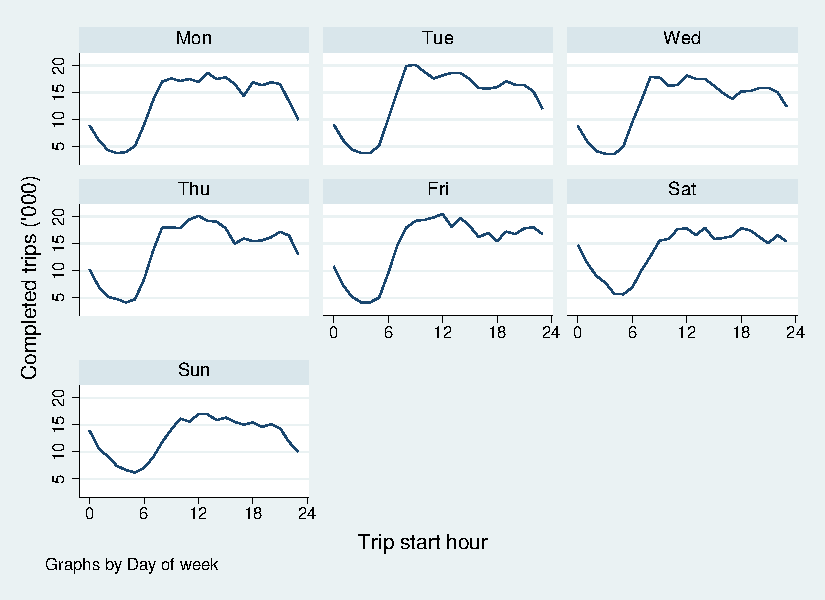
\includegraphics[width=0.8\linewidth]{./fg/completedtripsdow.pdf}
	\caption{Average hourly completed trips by day of week and trip start hour}
	\label{fg:trips}
\end{figure}

\begin{figure}
	\centering
	%	\includegraphics[width=0.8\linewidth]{./fg/cancellationsdow.pdf}
	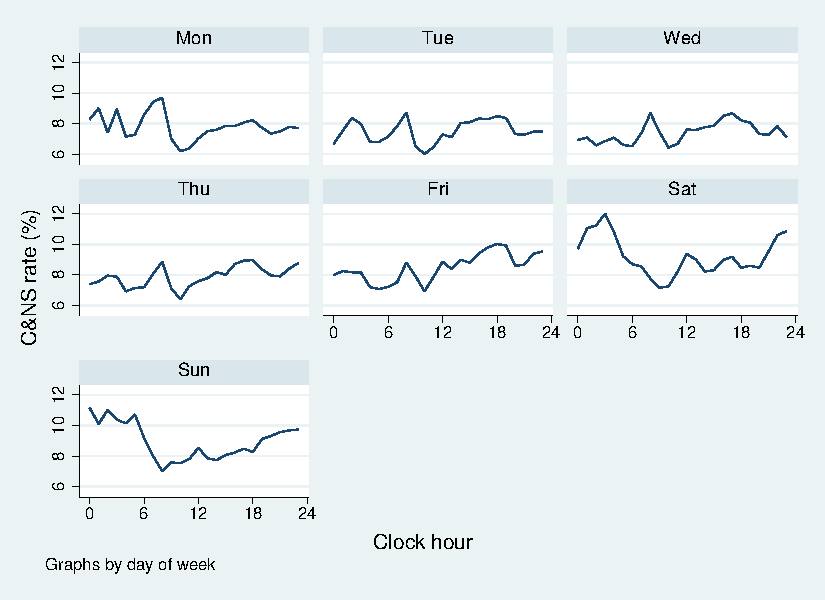
\includegraphics[width=0.8\linewidth]{./fg/cns_pct_dow.pdf}
	\caption{Percentage of cancellations and no-shows over total hourly bookings by day of week and hour of day}
	\label{fg:cancellations}
\end{figure}

\FloatBarrier

%\begin{figure}
%	\centering
%	\includegraphics[width=0.8\linewidth]{./fg/quitbyhour.pdf}
%	\caption{Proportion of drivers stopping work: with and without C\&NSs}
%	\label{fg:quitbyhour}
%\end{figure}

\begin{figure}
	{\centering
	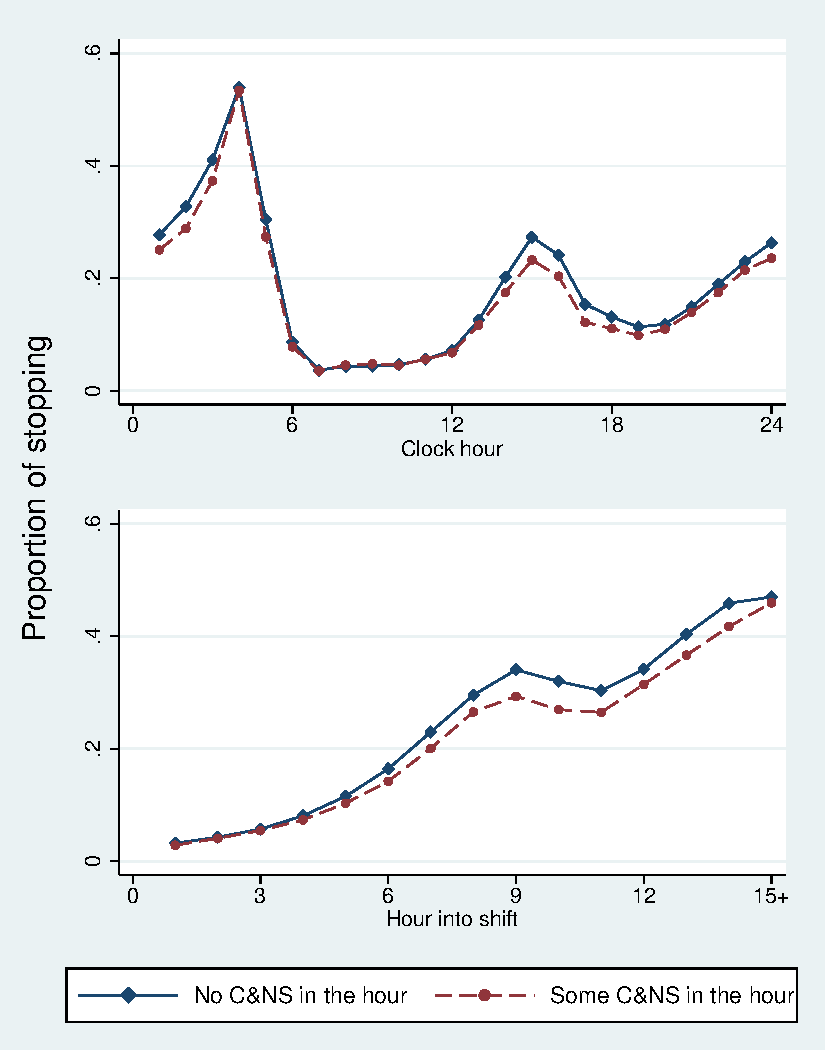
\includegraphics[width=0.8\linewidth]{./fg/modelfree_quit.pdf}
	\caption{Proportion of drivers who stop work: with and without C\&NSs}
	\label{fg:quitbyhour}}
	{\justifying\footnotesize\emph{Notes:} The top panel shows the proportion of drivers who stop work after each hour of the day over the total number of drivers who work in that hour. The bottom panel shows the proportion of drivers who stop work after a certain number of hours into the shift over the total number of drivers who for at least that number of hours into the shift. The solid lines are for driver-hours in which there are no C\&NSs. The dashed lines are for driver-hours in which there are some C\&NSs.}
\end{figure}

%\begin{figure}
%	\centering
%	\includegraphics[width=0.8\linewidth]{./fg/earningsbyhour.pdf}
%	\caption{Average hourly earnings: with and without C\&NSs in the previous hour}
%	\label{fg:earningsbyhour}
%\end{figure}


\begin{figure}
	{\centering
	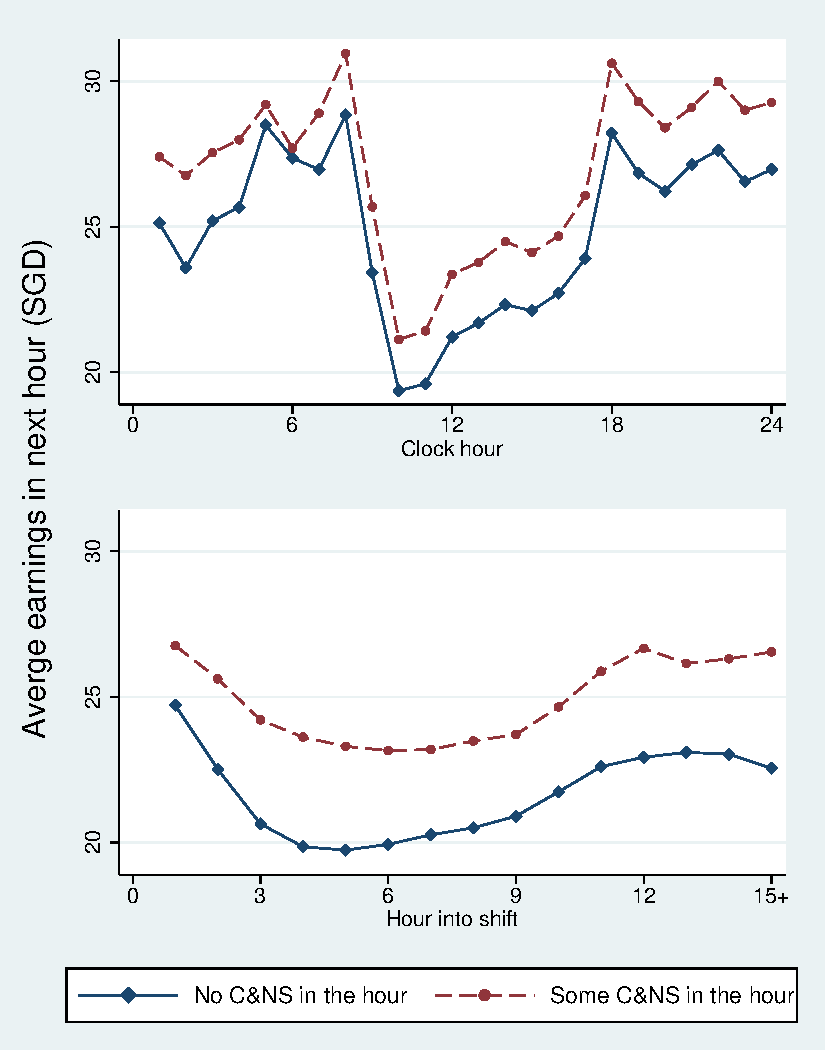
\includegraphics[width=0.8\linewidth]{./fg/modelfree_earnings.pdf}
	\caption{Average hourly earnings: with and without C\&NSs in the previous hour}
	\label{fg:earningsbyhour}}
	{\justifying\footnotesize\emph{Notes:} The figure shows drivers' average earning in the immediate hour following each hour of day (top panel) and hour into shift (bottom panel). The solid lines are for driver-hours in which there are no C\&NSs. The dashed lines are for driver-hours in which there are some C\&NSs.}
\end{figure}

\end{document}